\chapter{Sterile Neutrino Oscillation Inputs Within SBN}
\label{chap:osc_inputs}


\begin{figure}[!h]
    \centering
    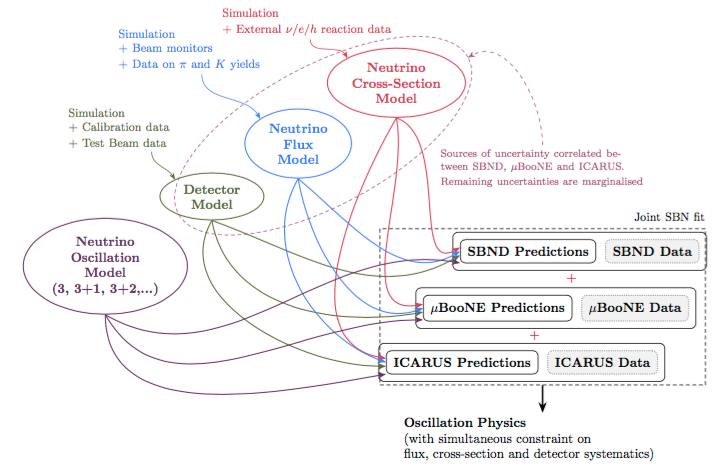
\includegraphics[width = \largefigwidth]{figures-chap5/valor_analysis.png}
    \caption{Overview of the SBN oscillation analysis paradigm. A given model for the neutrino oscillation, detector, neutrino flux and neutrino cross-section are combined with the appropriate data to give the prediction for the respective detector. Individual detector predictions may be combined to give an overall \gls{sbn} prediction. }
    \label{fig:analysis_paradigm}
\end{figure}

\section{Event Production}


\subsection{\texorpdfstring{\numu}{numu}}
\subsection{\texorpdfstring{\nue}{nue}}
The $\nue $ production followed the same steps described in section \ref{S:MCSamples:NumuProd}, however, in addition to generating an intrinsic $\nue$ sample, an oscillated $\numu \rightarrow \nue$ sample, a dirt sample and a cosmic sample were also produced. The oscillated sample is used to mimic the $\nue$ appearance signal whereas the dirt and cosmic samples are backgrounds. The other major background associated with a $\nue$ analysis involves $\numu$. A dedicated sample was not produced to emulate this, but instead the events from the $\numu$ production were also ran through the $\nue$ selection as mentioned in section \ref{S:NuESelection}. Table \ref{T:nue_production} outlines the number of events produced for each sample for each detector. The dirt events were produced with an additional filter at the generation stage which discarded any events where a shower above 10 MeV in the active volume was not present. This filter was used in order to remove any delta rays. Only about 1\% of dirt events would pass this filter so the number of dirt events used in the $\nue$ selection was $\sim$100,000. 


\begin{table}[h!]
\begin{tabular}{c cc}
Sample        & \begin{tabular}[c]{@{}c@{}}Events Produced\end{tabular} \\ \hline

Intrinsic $\nue$ & $\sim$1,000,000      \\
Oscillated $\nu$ & $\sim$1,000,000      \\
$\numu$          & {See $\nu_{\mu}$ sample}  \\
Dirt          & $\sim$10,000,000        \\
Cosmic\_Dirt  & $\sim$100,000             

\end{tabular}
\caption{The number of events initially produced for each sample in each of the three SBN detectors as part of the $\nue$ analysis.}
\end{table}\label{T:nue_production}


\section{\texorpdfstring{$\nu_\mu$ and $\nu_e$ Selections}{numu and nue Selections}}
Link in with Energy Reco. section

\section{Reaction Modes}
\subsection{Fine}

% Fine reaction modes
\begin{table}[t!]
  \renewcommand{\arraystretch}{1.6}
  \begin{tabular}{>{\centering\arraybackslash}m{4cm} 
                  >{\centering\arraybackslash}m{4cm}
                  >{\centering\arraybackslash}m{4cm}}
  
    \toprule
    \multicolumn{3}{c}{\textit{Fine Reaction Modes}} \\
    $\numu$, $\numubar$ & $\nue$, $\nuebar$ & $\numu \rightarrow \nue, \numubar \rightarrow \nuebar$ \\
    \midrule
    CC QE                      & CC QE                     & CC QE\\
    NC~Elastic                 & NC~Elastic                & CC MEC\\ 
    CC, NC MEC                 & CC, NC MEC                & CC 1$\pi^{\pm}$ \\  
    CC, NC 1$\pi^{\pm}$        & CC, NC 1$\pi^{\pm}$       & CC 1$\pi^{0}$ \\   
    CC, NC 1$\pi^{0}$          & CC, NC 1$\pi^{0}$         & CC 2$\pi^{\pm}$ \\   
    CC, NC 2$\pi^{\pm}$        & CC, NC 2$\pi^{\pm}$       & CC 2$\pi^{0}$i \\   
    CC, NC 2$\pi^{0}$          & CC, NC 2$\pi^{0}$         & CC Coh \\   
    CC, NC $\pi^{\pm}\pi^{0}$  & CC, NC $\pi^{\pm}\pi^{0}$ & Elastic Scattering \\   
    CC, NC Coh                 & CC, NC Coh                & CC Other \\  
    CC, NC Elastic Scattering  & CC+NC Elastic Scattering  \\  
    NC 1$\gamma$               & NC 1$\gamma$              \\  
    CC, NC Other               & CC, NC Other              \\  
    \hdashline
    \multicolumn{3}{c}{\textit{Cosmic \& Dirt}} \\
    \bottomrule

  \end{tabular}
  \caption[Fine Reaction Modes]{The complete list of reaction modes considered in an \gls{sbn} analysis.}
  \label{table:fine_reac_modes}
\end{table}




\subsection{Coarse}
% Coarse reaction modes
\begin{table}[t!]
  \begin{tabular}{>{\centering\arraybackslash}m{4cm} 
    >{\centering\arraybackslash}m{4cm}}
  
    \toprule
    \multicolumn{2}{c}{\textit{Coarse Reaction Modes}} \\
    $\numu$, $\numubar$ & $\nue$, $\nuebar$ \\
    \midrule
    $\numu$ CC QE          & \nue CC QE          \\ 
    $\numu$ CC MEC         & \nue CC MEC         \\ 
    $\numu$ CC 1$\pi$      & \nue CC 1$\pi$      \\ 
    $\numu$ CC 2$\pi$      & \nue CC 2$\pi$      \\ 
    $\numu$ CC Other       & \nue CC Other       \\ 
    $\numubar$ CC          & \nuebar CC          \\
    $\nue$ \& $\nuebar$ CC & \numu CC            \\
    NC                     & \numubar CC         \\
    \textit{Cosmic}        & Oscillated \nue CC  \\
    \textit{Dirt}          & NC 0\pi             \\
                           & NC Other            \\
                           & \textit{Cosmic}     \\
                           & \textit{Dirt}       \\
    \bottomrule

  \end{tabular}
  \caption[Coarse Reaction Modes]{The \textit{coarse} reaction modes used for both the \numu and \nue channels. These are broader definition of the reaction modes where one or more of the \textit{fine} reaction modes listed in \TableRef{table:fine_reac_modes} would come under the umbrella of a given coarse reaction mode.}
  \label{table:coarse_reac_modes}
\end{table}

\clearpage
\section{Flux Systematics}\label{sec:flux_syst}
\subsection*{Optical Flux Systematics}
The optical flux systematics are comprised of two parameters; the \textit{skin effect} and the \textit{horn current}. The horn current parameter is simply the uncertainty of the supplied current to the focusing horn. Since the current is linked to the focusing properties of the horn, uncertainty on the current leads to an uncertainty on the neutrino flux. The focusing horn is surrounded by a conductor where currents travel on the surface of the conductor. The skin effect is a measure of how much these surface currents penetrate into the conductor which in turn effect the internal fields of the conductor. Therefore, due to the skin effect, the strength of the magnetic field that particles propagating through the horn experience may vary \cite{BNB_flux}.

\begin{table}[!h]
  \renewcommand{\arraystretch}{1.4}    
  \begin{tabular}{p{2.5cm} p{10cm} p{2cm}}

    \toprule
    Parameter & Description & Uncertainty \\ 
    \midrule

    $f_{SkinEffect}$  & Depth that the current penetrates the horn conductor & $<18 \%$\\

    $f_{HornCurrent}$ & Current running in the horn conductor & $\pm 0.6 \%$\\
    \bottomrule

  \end{tabular}
  \caption[Optical, beam focusing flux systematic parameters]{Optical systematic flux uncertainties associated with the current in the horn\cite{BNB_flux}.}
  \label{}
\end{table}
\subsection*{Secondary Hadron Interaction Cross-Sections}
The proton interaction rate in \gls{bnb} target is largely dependent on the hadronic cross-sections with the beryllium target and aluminium horn. These cross-sections are divided into three categories; elastic scattering, quasi-elastic scattering and inelastic scattering. The total cross-section, $\sigma_{TOT}$, is defined as the sum of the elastic, $\sigma_{EL}$ and inelastic, $\sigma_{INEL}$, cross-sections. The quasi-elastic cross-section, $\sigma_{QE}$, is a subset of the  $\sigma_{INEL}$ cross-section. The $\sigma_{TOT}$ variations are based on comparing calculations with neutron-nucleus measurements. The model describing $\sigma_{TOT}$ is assumed to work sufficiently well for $\pi^{\pm}$-nucleus interactions and is extended to include these interactions in addition to all nucleon-nucleus interactions. $\sigma_{INEL}$ is estimated directly from the available data and the deviations are therefore noticeably smaller than for $\sigma_{TOT}$. The variations are chosen to encompass the uncertainties in the measurements. $\sigma_{QEL}$ variations are again estimated from a combination of the available date and models. Finally, the linked relationship between the different cross-section is considered such that: 1) If  $\sigma_{INEL}$ is fixed, a variation in $\sigma_{TOT}$ will result in a variation in $\sigma_{EL}$. 2) If $\sigma_{INEL}$ is varied, the relative contribution from $\sigma_{INEL}$ and $\sigma_{EL}$ to  $\sigma_{TOT}$ (which remains constant) will vary. 3) If $\sigma_{QEL}$ is varied, the relative contribution from other inelastic process to $\sigma_{INEL}$ (which remains constant) will vary \cite{BNB_flux}.

The above approach is applied for both beryllium and aluminium nuclei and the uncertainty associated with the total, quasi-elastic and inelastic cross-sections for both nucleons and pions for the two nuclei are shown in \TableRef{table:secondary_hadron_interaction_xsec}.

\begin{table}[!h]
  \renewcommand{\arraystretch}{1.4}    
  \begin{tabular}{p{2.5cm} p{9.2cm} p{1.2cm} p{1.2cm}}
    \toprule
    \multirow{2}{*}{Parameter} & \multirow{2}{*}{Description} & \multicolumn{2}{c}{Uncertainty} \\
    && \multicolumn{1}{c}{Be} & \multicolumn{1}{c}{Al} \\
    \midrule

    $f_{\sigma_{INEL}^{N}}$   & Secondary inelastic nucleon cross-section in the target (Be) and horn (Al) & $\pm 5 \%$ & $\pm 10 \%$\\
                            
    $f_{\sigma_{QE}^{N}}$     & Secondary quasi-elastic nucleon cross-section in the target (Be) and horn (Al) & $\pm 20 \%$ & $\pm 45 \%$\\
                            
    $f_{\sigma_{TOT}^{N}}$    & Secondary total nucleon cross-section in the target (Be) and horn (Al) & $\pm 15 \%$ & $\pm 25 \%$\\

    $f_{\sigma_{INEL}^{\pi}}$ & Secondary inelastic pion cross-section in the target (Be) and horn (Al) & $\pm 10 \% $ & $\pm 20 \% $\\
                          
    $f_{\sigma_{QE}^{\pi}}$   & Secondary quasi-elastic pion cross-section in the target (Be) and horn (Al) & $\pm 11.2 \% $ & $\pm 25.9 \% $\\
                          
    $f_{\sigma_{TOT}^{\pi}}$  & Secondary total pion cross-section in the target (Be) and horn (Al) & $\pm 11.9 \%$ & $\pm 28.7 \%$\\
    \bottomrule
  \end{tabular}
  \caption[Hadronic secondary interaction flux systematic parameters]{The systematic uncertainties associated with secondary hadron interaction cross-sections in both the horn (Aluminium) and the target (Beryllium) \cite{SBN_Proposal}}.
  \label{table:secondary_hadron_interaction_xsec}
\end{table}


\subsection*{Hadronic Neutrino Production Flux Uncertainties}
The majority of neutrinos in the \gls{bnb} are due to decaying particles which are a result of protons interacting with beryllium target. Understanding the neutrino flux therefore relies on understanding the production of the particles decaying to neutrinos, which are predominately pions for \numu and kaons for \nue (plus the decay of muons which in turn are produced in the meson decays). 

The Sanford-Wang parameterisation is used to estimate the $\pi^{\pm}$ production. It depends on the meson momentum, \textit{p}, and angle relative to the incident proton, \textit{\theta}, and also the proton momentum, $p_B$. The parametrisation is given by

\begin{equation}
  \hspace{-0.35cm}
  \label{eq:SW}
  \frac{d^{2}\sigma}{dpd\theta} = 
  c_{1}p^{c_{2}} 
  \left( 1 - \frac{p}{p_{B} -c_{9}} \right)
  \exp \left( -c_{3} \frac{p^{c_{4}}}{p_{B}^{c_{5}}} - c_{6}\theta(p - p_{B}c_{7}cos^{c_{8}}\theta) \right),
\end{equation}

where parameters $c_{1 \rightarrow 9}$ are determined from the HARP (8.89 GeV/c), BNL E910 (6.4 GeV/c) and BNL E910 (12.3 GeV/c) experiments \cite{BNB_flux}.

No $k^+$ production rates exist for proton-beryllium interactions at 8.89 GeV/c which is the primary \gls{bnb} operating momentum. To estimate the $k^+$ production rate at the \gls{bnb} momentum, Feynman scaling is used to extrapolate the rate from production rates at nearby energies \cite{BNB_flux}.

The major contribution that the $k^0$ makes to the BNB flux is from the decay of the $k^0_L$. The $k^0$ that are produced via strong interactions have equal contents of $k^0_L$ and $k^0_s$, therefore the production rate of $k^0_L$ can be inferred from knowing the production rate of $k^0_s$. The Sanford-Wang parametrisation is again used to estimate the production cross-section by combining data from the BNL E910 experiment at 12.3 GeV/c and 17.5 GeV/c and the KEK experiment at 12.3 GeV/c.

For the $k^-$, there is minimal production data available, therefore simulations are used exclusively. The rate and spectrum of the $k^-$ are estimated by simulating 8.89 GeV/c proton-beryllium interactions \cite{BNB_flux}.

\begin{table}[!h]
  \renewcommand{\arraystretch}{1.4}    
  \begin{tabular}{p{2cm} p{6.0cm} p{1.2cm} p{1.2cm} p{1.2cm} p{1.2cm}}
    \toprule
    \multirow{2}{*}{Parameter} & \multirow{2}{*}{Description} & \multicolumn{4}{c}{Uncertainty} \\
    && \multicolumn{1}{c}{$\nu_{\mu}$} & \multicolumn{1}{c}{$\bar{\nu}_{\mu}$} & \multicolumn{1}{c}{$\nu_{e}$} & \multicolumn{1}{c}{$\bar{\nu}_{e}$} \\
    \midrule

    $f_{\pi^{+}}$ & $\nu$ production mechanism: $\pi^{+}$ & $ \pm 11.7 \%$ & $ \pm 1.0 \%$ & $ \pm 10.7 \%$ & $ \pm 0.03 \%$ \\

    $f_{\pi^{-}}$ & $\nu$ production mechanism: $\pi^{-}$ & $ \pm 0.0 \%$ & $ \pm 11.6 \%$ & $ \pm 0.0 \%$ & $ \pm 3.0 \%$ \\

    $f_{K^{+}}$   & $\nu$ production mechanism: $K^{+}$ & $ \pm 0.2 \%$ & $ \pm 0.1 \%$ & $ \pm 2.0 \%$ & $ \pm 0.1 \%$ \\
                  
    $f_{K^{-}}$   & $\nu$ production mechanism: $K^{-}$ & $ \pm 0.0 \%$ & $ \pm 0.4 \%$ & $ \pm 0.0 \%$ & $ \pm 3.0 \%$ \\
                  
    $f_{K^{0}}$   & $\nu$ production mechanism: $K^{0}$ & $ \pm 0.0 \%$ & $ \pm 0.3 \%$ & $ \pm 2.3 \%$ & $ \pm 21.4 \%$ \\

    \bottomrule
  \end{tabular}
  \caption[Hadronic neutrino production flux systematic parameters]{Hadronic neutrino production systematic flux uncertainties \cite{BNB_flux_TN}.}
  \label{}
\end{table}

\subsection*{BNB POT Normalisation}
The intensity of the proton beam is monitored by two toroids and it has been found that the two toroids agree with one another to within 2\% \cite{BNB_flux}. An additional 2\% normalisation uncertainty is applied in order to account for this \gls{pot} accounting uncertainty. This uncertainty is set so that it is fully correlated between all analysis bins.








\clearpage
\section{Interaction Systematics}\label{sec:interaction_syst}
The uncertainties associated with neutrino interactions are provided by GENIE and are implemnted using the GENIE ReWeight package. This is the case for all the interaction systematics considered here except for the \gls{mec} systematic (see \SectionRef{sec:MEC_uncertainty}). The GENIE reweighting scheme works as follows: For each quantity, \textit{P}, which has an associated uncertainty, a systematic parameter, $x_P$ is introduced. Varying $x_P$ will modify, \textit{P} such that
\begin{equation}
    P \rightarrow P' = P (1 + x_P . \frac{\delta P}{P}),
\end{equation}\label{eqn:genie_reweight}
where $\delta P$ represents the standard deviation of \textit{P}. It follows from \EquationRef{eqn:genie_reweight} that for a $x_P = 0$, $P' = P$ and for $x_P = \pm 1$, $P' = P \pm \delta P$.

The two main types of interaction systematics considered in this analysis are cross-section and intranuclear hadron transport model uncertainties. 

\section*{Neutrino Cross-Section uncertainties}
\begin{equation}
    w_\sigma^{evt} = \left(\frac{d^n\sigma'_\nu}{dK^n}\right)\Bigg/\left(\frac{d^n\sigma_\nu}{dK^n}\right)
\end{equation}

$\frac{d^n\sigma'_\nu}{dK^n}$ is the differential cross-section with varied physics parameters and  $\frac{d^n\sigma_\nu}{dK^n}$ is the nominal differential cross-section with $K^n$ being the kinematical phase space in both cases.  

\cite{GENIE_manual}

\subsection*{\textit{Proposal} Interaction Systematics}
\begin{table}[h!]
    \renewcommand{\arraystretch}{1.4}
    \begin{tabular}{p{1.8cm} p{10cm}>{\centering\arraybackslash}p{ 2.2cm}}
        \toprule
         Parameter & Description & $\delta P / P$ \\
        \midrule
         $f_{M_{A}^{CCQE}}$  & Axial mass for CC quasi-elastic & -15\% +25\% \\
         
         $f_{M_{A}^{CCRes}}$ & Axial mass for CC resonance neutrino production & $\pm 20\%$ \\
         
         $f_{M_{A}^{NCRes}}$ & Axial mass for NC resonance neutrino production & $\pm 20\%$ \\
         
         $f_{NC}$              & Additional error on NC/CC ratio & $\pm 25\%$ \\
         
         $f_{nR_{\nu n}^{CC1\pi}}$ & Non-resonance bkg normalisation in $\nu n$ CC1$\pi$ reactions & $\pm 50\%$ \\
         
         $f_{nR_{\nu p}^{CC1\pi}}$ & Non-resonance bkg normalisation in $\nu p$ CC1$\pi$ reactions & $\pm 50\%$ \\
         
         $f_{nR_{\nu n}^{CC2\pi}}$ & Non-resonance bkg normalisation in $\nu n$ CC2$\pi$ reactions & $\pm 50\%$ \\
         
         $f_{nR_{\nu p}^{CC2\pi}}$ & Non-resonance bkg normalisation in $\nu p$ CC2$\pi$ reactions & $\pm 50\%$ \\
         
         $f_{nR_{\bar{\nu} n}^{CC1\pi}}$ & Non-resonance bkg normalisation in $\bar{\nu} n$ CC1$\pi$ reactions & $\pm 50\%$ \\
         
         $f_{nR_{\bar{\nu} p}^{CC1\pi}}$ & Non-resonance bkg normalisation in $\bar{\nu} p$ CC1$\pi$ reactions & $\pm 50\%$ \\
         
         $f_{nR_{\bar{\nu} n}^{CC2\pi}}$ & Non-resonance bkg normalisation in $\bar{\nu} n$ CC2$\pi$ reactions & $\pm 50\%$ \\
         
         $f_{nR_{\bar{\nu} p}^{CC2\pi}}$ & Non-resonance bkg normalisation in $\bar{\nu} p$ CC2$\pi$ reactions & $\pm 50\%$ \\
        
         $f_{nR_{\nu n}^{NC1\pi}}$ & Non-resonance bkg normalisation in $\nu n$ NC1$\pi$ reactions & $\pm 50\%$ \\
         
         $f_{nR_{\nu p}^{NC1\pi}}$ & Non-resonance bkg normalisation in $\nu p$ NC1$\pi$ reactions & $\pm 50\%$ \\
         
         $f_{nR_{\nu n}^{NC2\pi}}$ & Non-resonance bkg normalisation in $\nu n$ NC2$\pi$ reactions & $\pm 50\%$ \\
         
         $f_{nR_{\nu p}^{NC2\pi}}$ & Non-resonance bkg normalisation in $\nu p$ NC2$\pi$ reactions & $\pm 50\%$ \\
         
         $f_{nR_{\bar{\nu} n}^{NC1\pi}}$ & Non-resonance bkg normalisation in $\bar{\nu} n$ NC1$\pi$ reactions & $\pm 50\%$ \\
         
         $f_{nR_{\bar{\nu} p}^{NC1\pi}}$ & Non-resonance bkg normalisation in $\bar{\nu} p$ NC1$\pi$ reactions & $\pm 50\%$ \\
         
         $f_{nR_{\bar{\nu} n}^{NC2\pi}}$ & Non-resonance bkg normalisation in $\bar{\nu} n$ NC2$\pi$ reactions & $\pm 50\%$ \\
         
         $f_{nR_{\bar{\nu} p}^{NC2\pi}}$ & Non-resonance bkg normalisation in $\bar{\nu} p$ NC2$\pi$ reactions & $\pm 50\%$ \\
        
        \bottomrule
        
    \end{tabular}
    \caption[SBN proposal interaction cross-section systematic parameters]{GENIE interaction cross-section systematics considered in \gls{sbn} as part of the \textit{proposal} set of systematics. \cite{GENIE_manual}.}
    \label{}
\end{table}


\subsection*{\textit{Modern} Interaction Systematics}

\begin{table}[h!]
    \renewcommand{\arraystretch}{1.4}
    \begin{tabular}{p{1.8cm} p{10cm}>{\centering\arraybackslash}p{ 2.2cm}}
        \toprule
         Parameter & Description & $\delta P / P$ \\
        \midrule
         $f_{M_{A}^{NCEl}}$  & Axial mass for NC elastic & $\pm 25\%$ \\
         
         $f_{\eta^{NCEl}}$    & Strange axial form factor for NC elastic & $\pm 30\%$ \\
        
         %$f_{2p2h}$          & Normalisation uncertainty for 2p2h interactions & $\pm 100\%$ \\
         
         $f_{M_{V}^{CCRes}}$ & Vector mass for CC resonance neutrino production & $\pm 10\%$ \\
         
         $f_{M_{V}^{NCRes}}$ & Vector mass for NC resonance neutrino production & $\pm 10\%$ \\
         
         $f_{A_{HT}}$          & Higher-twist parameter A for NC and CC DIS events & $\pm 25\%$ \\
         
         $f_{B_{HT}}$          & Higher-twist parameter B for NC and CC DIS events & $\pm 25\%$ \\
         
         $f_{C_{v1u}}$         & Valence p.d.f. correction factor $C_{v1u}$ for DIS events & $\pm 30\%$ \\
         
         $f_{C_{v2u}}$         & Valence p.d.f. correction factor $C_{v2u}$ for DIS events & $\pm 40\%$ \\
         
         $f_{M_{A}^{Coh}}$     & Axial mass for NC and CC coherent pion production & $ \pm 50 \%$ \\
         
         $f_{R_{0}^{Coh}}$     & Nuclear size parameter controlling $\pi$ absorption & $\pm 20 \%$ \\
        
        $f_{\Delta\rightarrow N\gamma}$   & Branching ratio for $\Delta$ radiative decay & $\pm 50 \%$ \\
        
        \bottomrule
        
    \end{tabular}
    \caption[Modern interaction cross-section systematic parameters]{GENIE interaction cross-section systematics considered in \gls{sbn} as part of the \textit{modern} set of systematics \cite{GENIE_manual}.}

    \label{}
\end{table}


\begin{table}[!h]
    \renewcommand{\arraystretch}{1.4}
    \begin{tabular}{p{1.8cm} p{11.4cm} p{1.2cm}}
        \toprule
         Parameter & Description & $\delta P / P$ \\
        \midrule
        
         $f_{\lambda_{\pi}}$   & Intranuclear mean free path for pions & $ \pm 20 \% $ \\
        
         $f_{R^{CEx}_{\pi}}$    & Intranuclear charge exchange rescattering fraction for pions & $ \pm 50 \% $ \\
        
         $f_{R^{Inel}_{\pi}}$   & Intranuclear inelastic rescattering fraction for pions & $ \pm 40 \% $ \\
        
         $f_{R^{\pi}_{\pi}}$    & Intranuclear pion-production rescattering fraction for pions & $ \pm 20 \% $ \\
        
         $f_{R^{Abs}_{\pi}}$    & Intranuclear absorption fraction for pions & $ \pm 20 \% $ \\
        
         $f_{\lambda_{N}}$     & Intranuclear mean free path for nucleons & $ \pm 20 \% $ \\
        
         $f_{R^{CEx}_{N}}$      & Intranuclear charge exchange rescattering fraction for nucleons & $ \pm 50 \%$ \\
        
         $f_{R^{Inel}_{N}}$     & Intranuclear inelastic rescattering fraction for nucleons & $ \pm 40 \% $ \\
        
         $f_{R^{\pi}_{N}}$      & Intranuclear pion-production rescattering fraction for nucleons & $ \pm 20 \% $ \\
        
         $f_{R^{Abs}_{N}}$      & Intranuclear absorption fraction for nucleons & $ \pm 20 \% $ \\

        \bottomrule
    \end{tabular}
    \caption[Intranuclear hadron transport systematic parameters]{\cite{GENIE_manual}}
    \label{}
\end{table}


\subsection*{MEC uncertainty}\label{sec:MEC_uncertainty}
A \gls{mec} uncertainty parameter which specifically affects \gls{mec} events is not included from the GENIE event generator since it was decided that the parameter was not sufficiently validated. Instead, a 100\% normalisation uncertainty is applied to all \gls{mec} events. The value of the uncertainty was chosen to be a 100\% (maximal) to ensure the effect of the \gls{mec} parameter would not be an underestimate. 



\clearpage
\section{Other Systematics}

Efficiency systematics and energy scale systematics are not implemented in the \textit{standard} analyses because there currently isn't a good handle on how to correctly quantify them. A rigorous scheme akin to those described in \SectionRef{sec:flux_syst} and \SectionRef{sec:interaction_syst} doesn't exist, so instead in-house methods have been developed which are described below.

\subsection{Efficiency Systematics}

The current scheme for implementing efficiency (detector) systematics into a fit is by use of a covariance matrix where each element is defined by the systematics outlined in  \TableRef{table:efficiency_systematics}. In general, we assume that a covariance matrix $\mathcal{M}_{ij}$ is comprised of both correlated uncertainties and uncorrelated uncertainties such that
\begin{equation}
    \mathcal{M}_{ij} = \mathcal{M}_{ij}^{corr} + \mathcal{M}_{ij}^{uncorr},
\end{equation}
where $\mathcal{M}_{ij}^{corr}$ is the correlated component and $\mathcal{M}_{ij}^{uncorr}$ is the uncorrelated component. For correlated uncertainties,
\begin{equation}
  \mathcal{M}_{ij}^{corr}=\begin{cases}
    \sigma_i^2, & \text{$i = j$}\\
    C_{ij} \sigma_i \sigma_j, & \text{$i \neq j$},
  \end{cases}
\end{equation}
where $C_{ij}$ represents the correlation between the off-diagonal elements and $\sigma_{i,j}$ is some percentage error associated with each systematic. In the case of fully correlated uncertainties, $C_{ij}$ reduces to one and $\sigma_i = \sigma_j$. For uncorrelated uncertainties,
\begin{equation}
  \mathcal{M}_{ij}^{uncorr}=\begin{cases}
    \sigma_i^{'2}, & \text{$i = j$}\\
    0, & \text{$i \neq j$},
  \end{cases}
\end{equation}
If any correlated errors are assumed to by fully correlated, $\mathcal{M}_{ij}$ will then have diagonal elements given by $\sigma_i^2 + \sigma_i^{'2}$ and off diagonal elements given by $\sigma_i^2$.

A set of example covariance matrices are shown in \FigureRef{fig:efficiency_cov_matrices}. The top left plot corresponds to a 10\% correlated error only. The remaining three plots all have a correlated error of 2\%, with some varying amounts of an uncorrelated error associated with each systematic. 

\begin{figure}
    \centering
    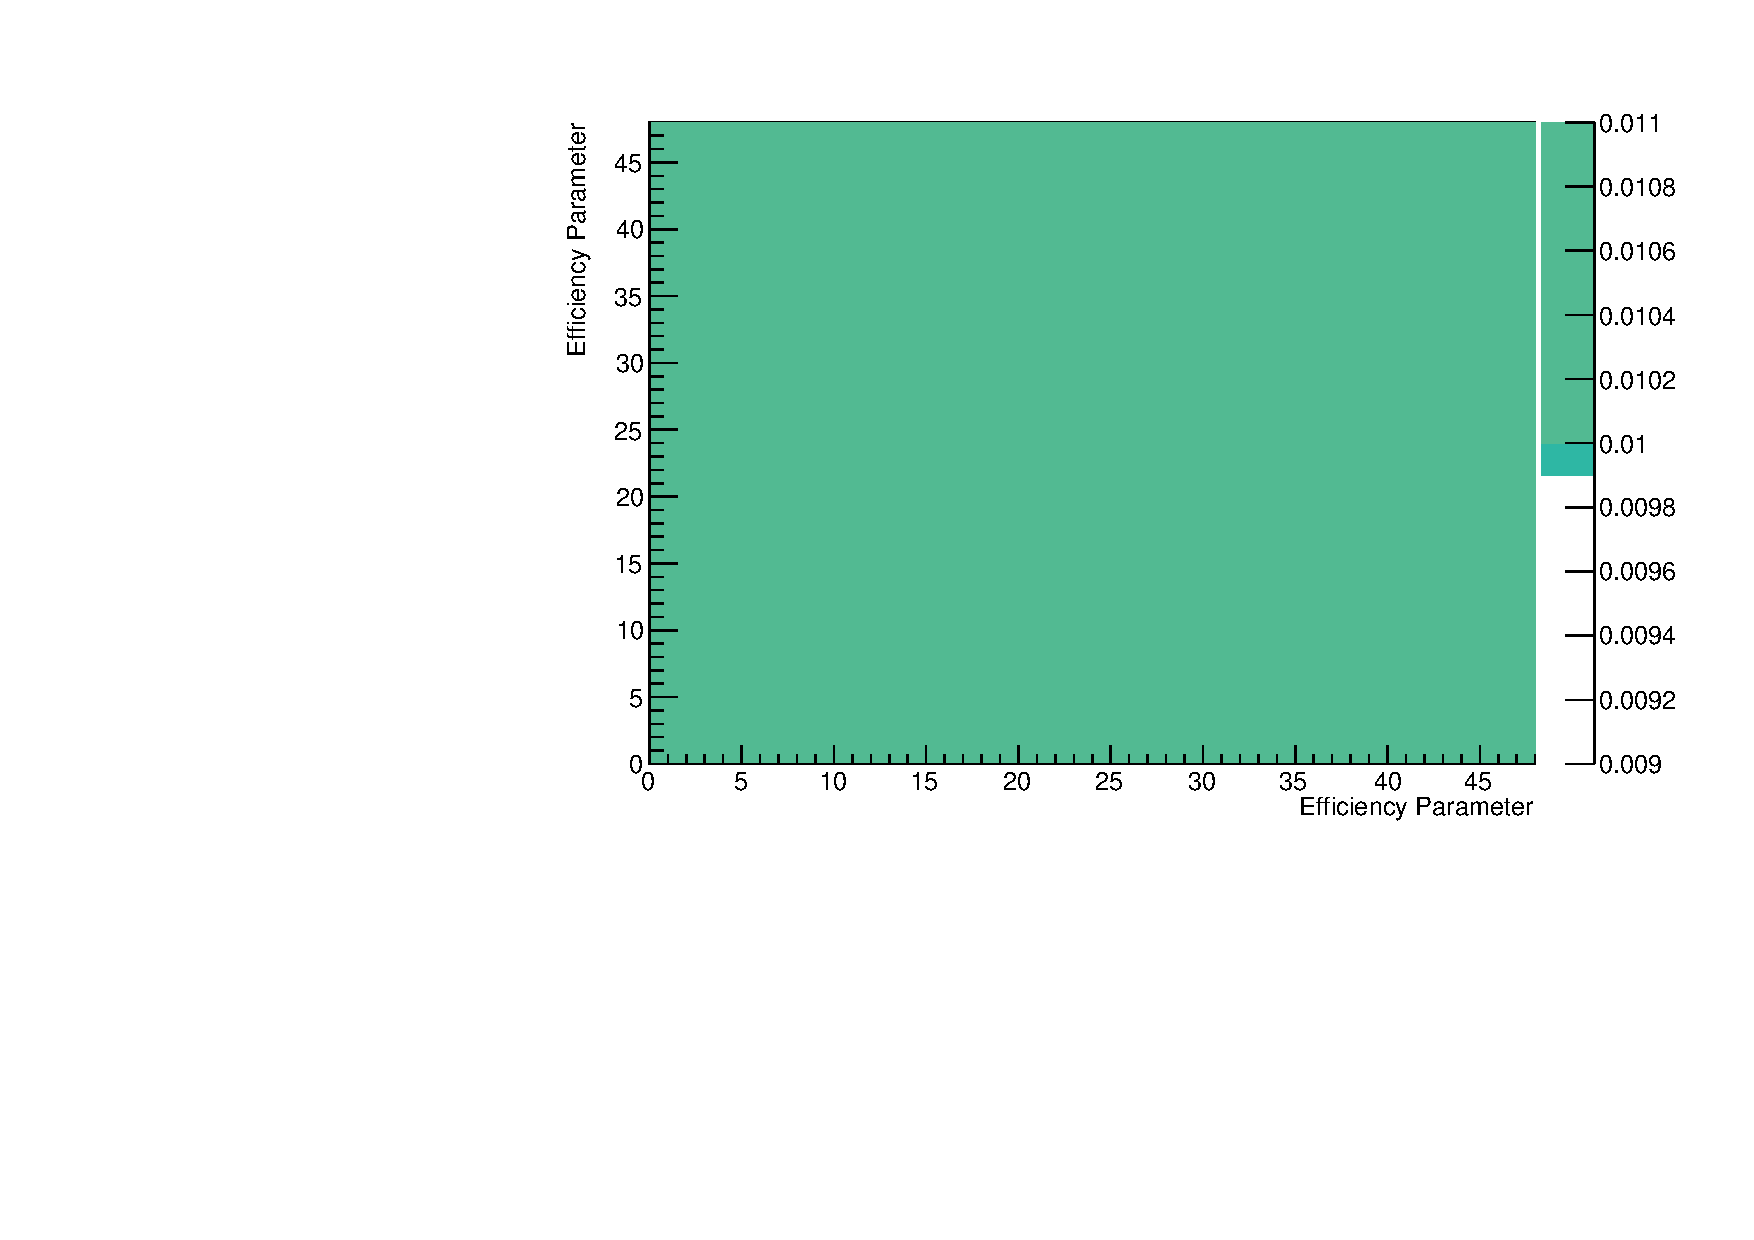
\includegraphics[width = 0.49\textwidth]{figures-chap5/efficiency_matrices/efficiency_error_matrix_48x48_type1_cor10.00pct.root.pdf}
    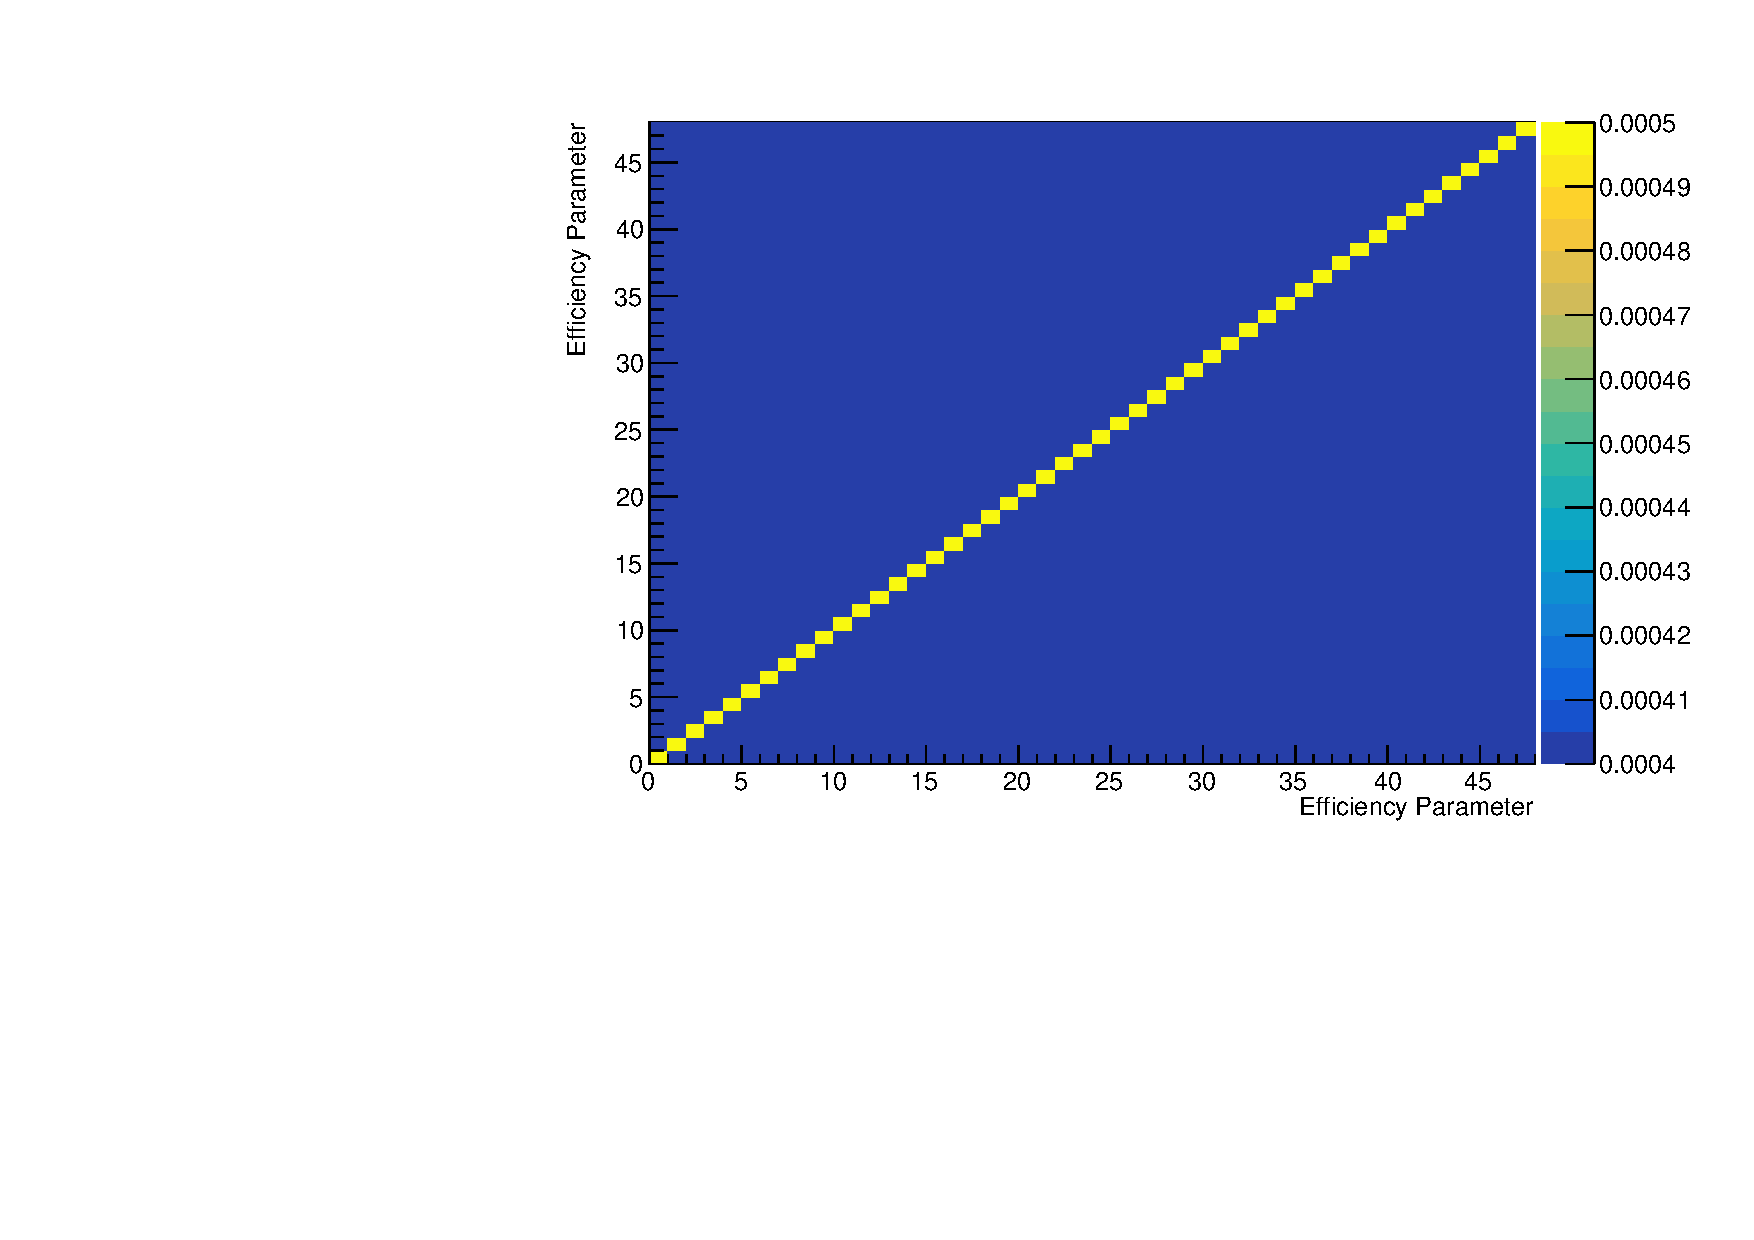
\includegraphics[width = 0.49\textwidth]{figures-chap5/efficiency_matrices/efficiency_error_matrix_48x48_type2_cor2.00pct_sbnduncor1.00pct_ubooneuncor1.00pct_icarusuncor1.00pct.root.pdf}
    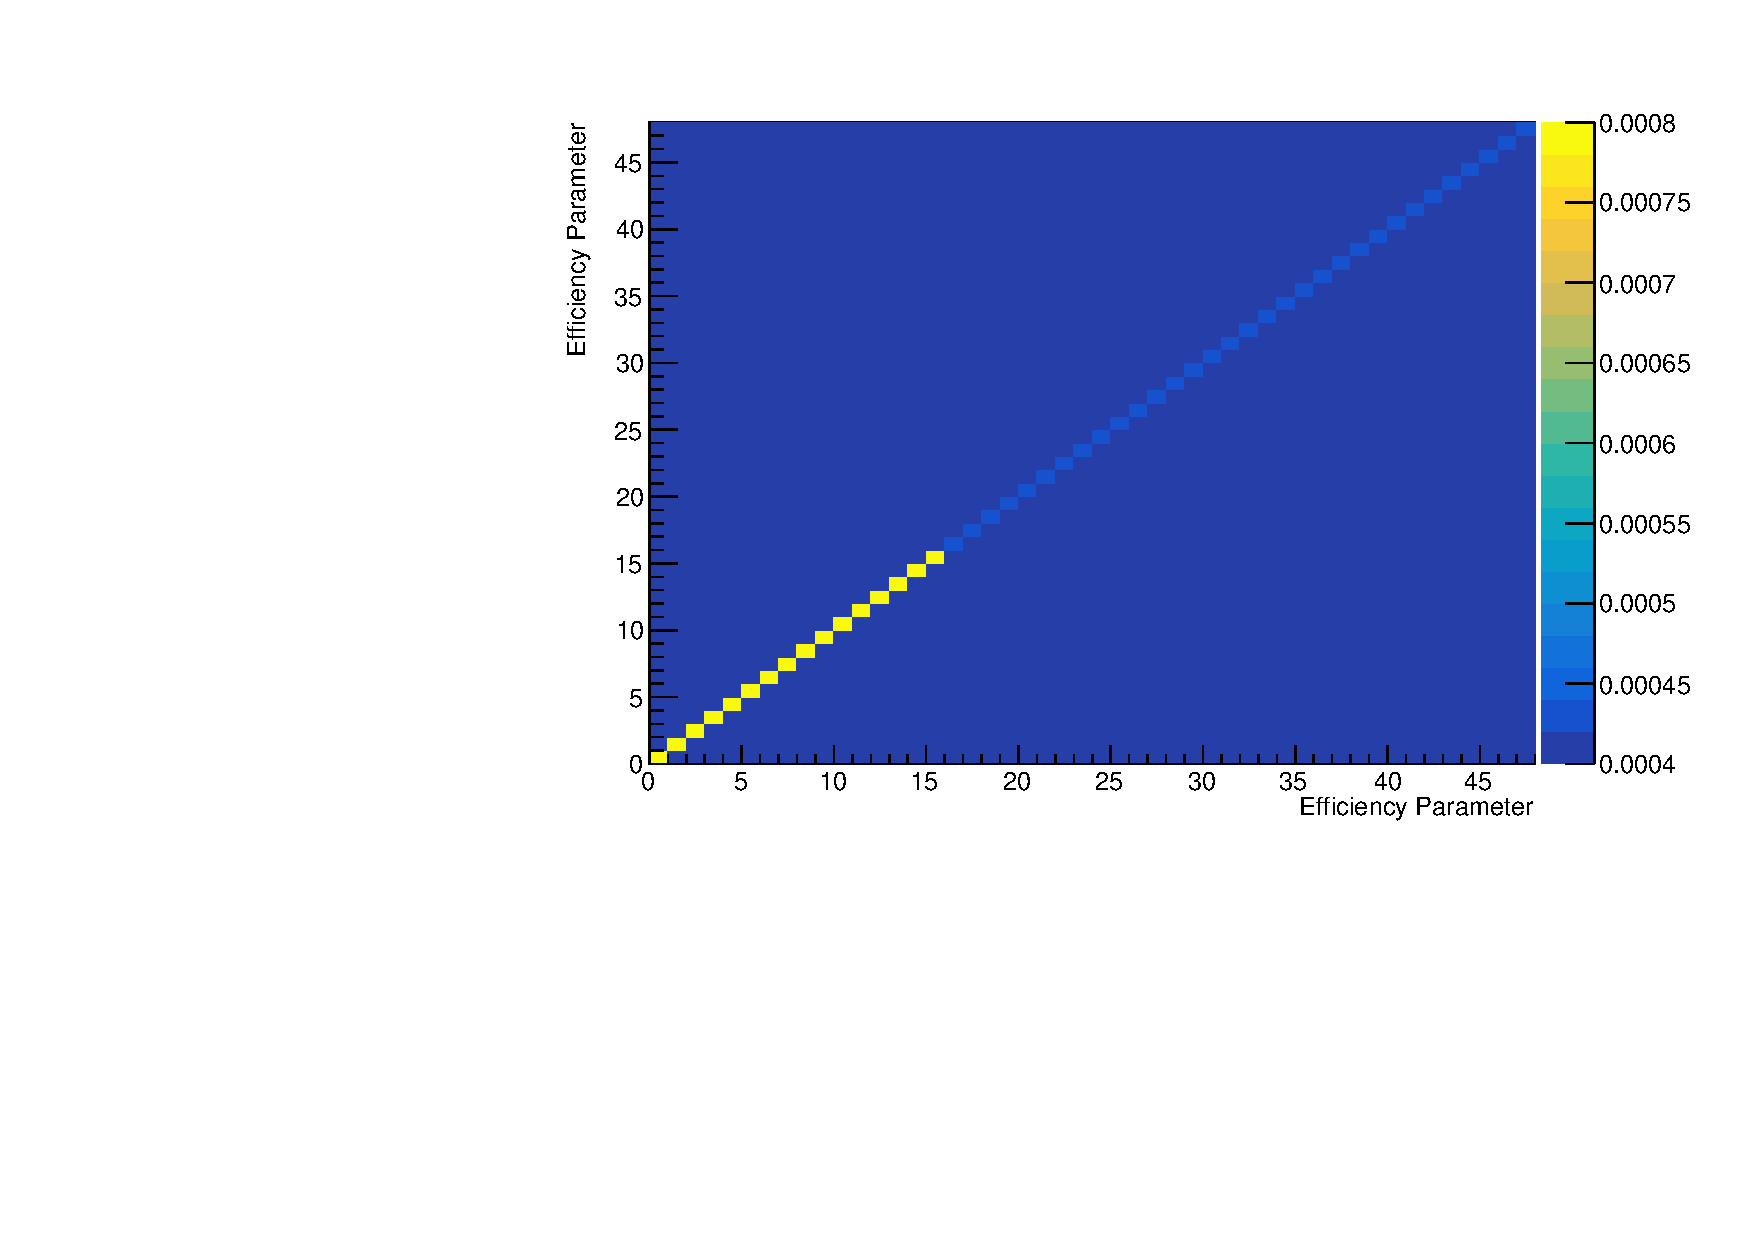
\includegraphics[width = 0.49\textwidth]{figures-chap5/efficiency_matrices/efficiency_error_matrix_48x48_type2_cor2.00pct_sbnduncor2.00pct_ubooneuncor0.50pct_icarusuncor0.50pct.root.pdf}
    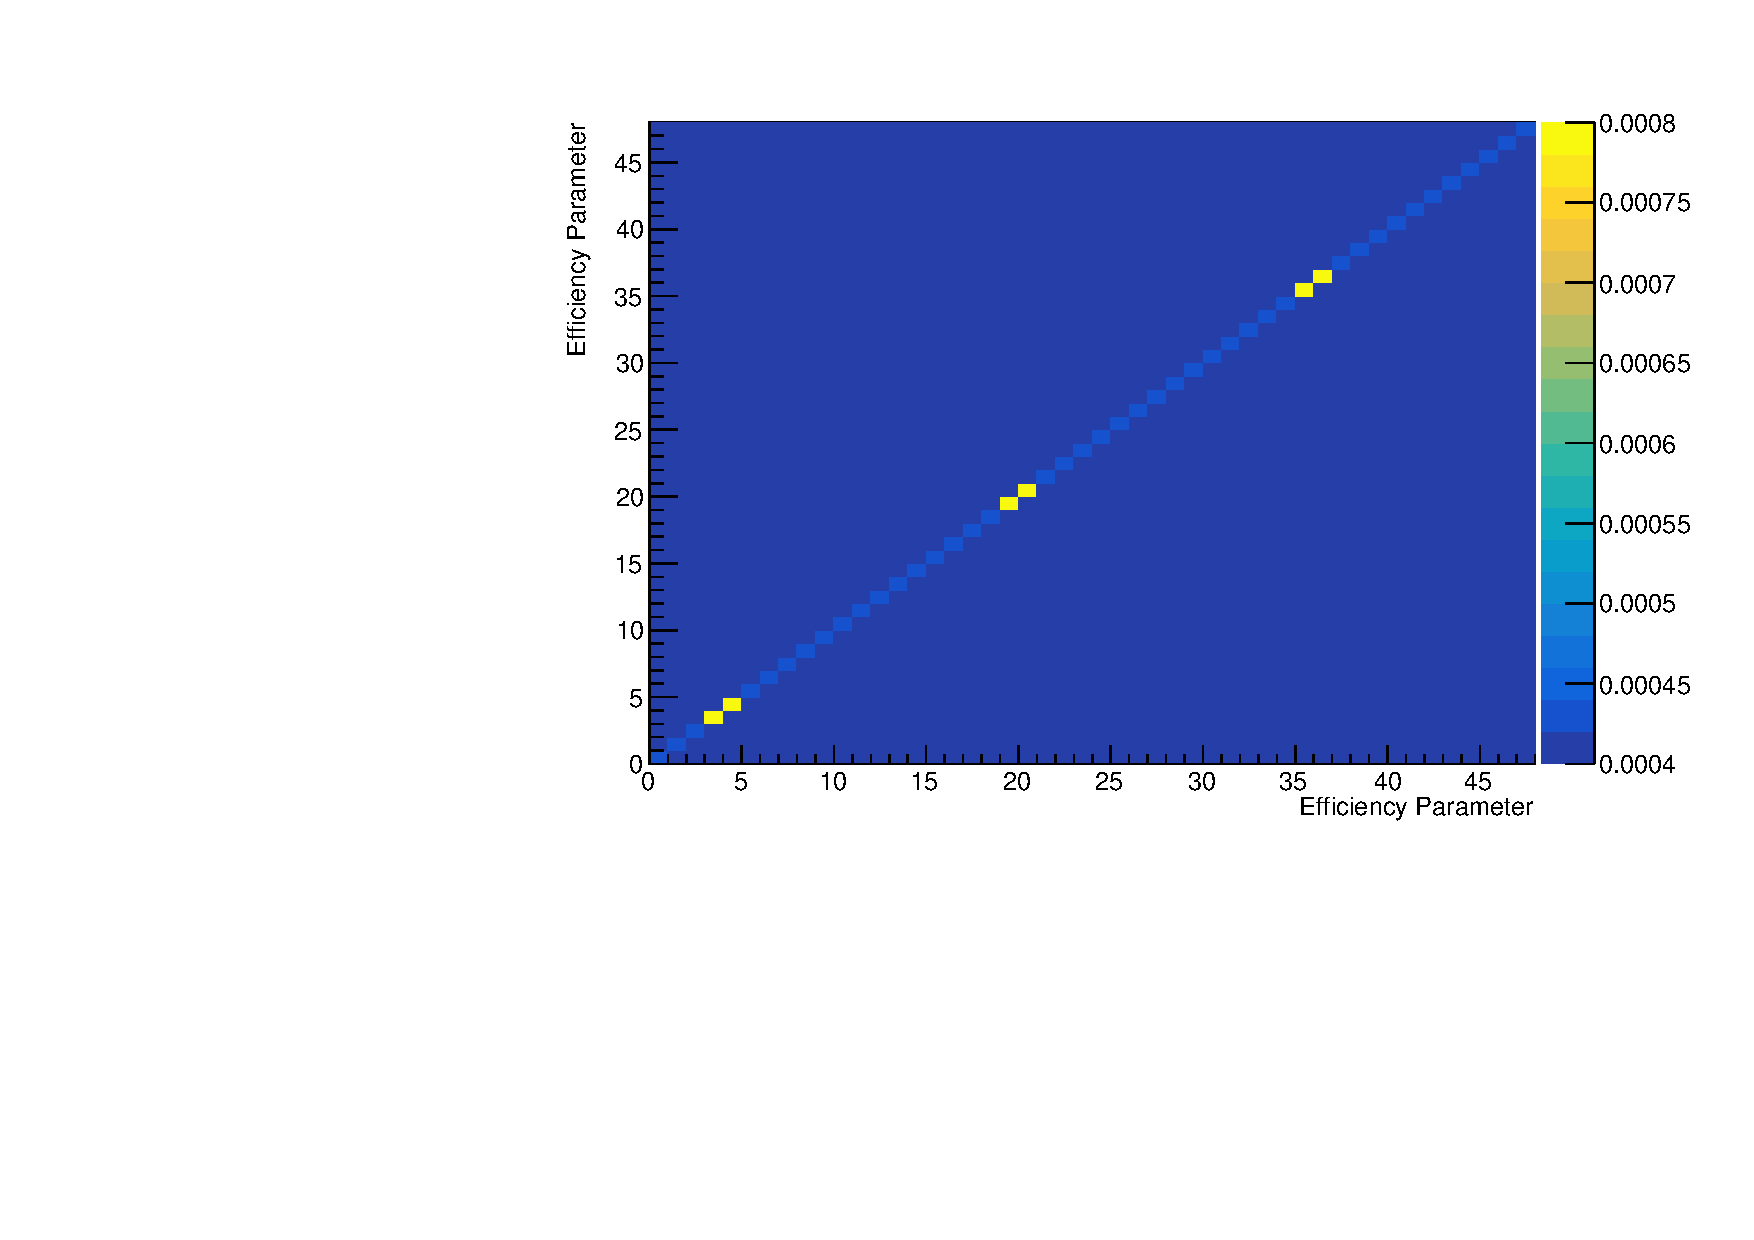
\includegraphics[width = 0.49\textwidth]{figures-chap5/efficiency_matrices/efficiency_error_matrix_48x48_type3_cor2.00pct_bulkuncor0.50pct_allpeakEnumuCCuncor2.00pct.root.pdf}
    \caption{Covariance matrices produced to investigate the effects of efficiency systamatics for the \numu disappearance channel. Top left: A 10\% fully correlated error only. Top right: A 2\% fully correlated error with an additional 1\% uncorrelated error across all bins. Bottom left: A 2\% fully correlated error with an additional 2\% uncorrelated error for all \gls{sbnd} bins and a 0.5\% uncorrelated error for all \gls{microboone} and \gls{icarus} bins. Bottom right: A 2\% fully correlated error with and additional 2\% uncorrelated error for the peak energy bins (0.6 - 1.0 GeV) in each detector and a 0.5\% uncorrelated error for all other bins.}
    \label{fig:efficiency_cov_matrices}
\end{figure}



\begin{table}[]
\begin{adjustbox}{width=\textwidth,center}
	\begin{tabular}{l lllll}
		\hline
		& \multicolumn{5}{c}{\textbf{Applies to}}                                                                                  \\
		\textbf{Systematic}    & \textbf{Beam} & \textbf{Detector} & \textbf{Sample}        & \textbf{Mode} & \textbf{Reco. energy bin edges}                            \\ \hline
		$f_0 - f_7$   & FHC  & SBND     & $\nu_{\mu}$CC-like & signal/$\nu_{\mu}$CC & \{0, 0.2, 0.4, 0.6, 0.8, 1.0, 1.5, 2.0, $\infty$\}      \\
		$f_8 - f_{13}$    & FHC  & SBND     & $\nu_{\mu}$CC-like   & bkg/NC               & \{0, 0.2, 0.4, 0.6, 0.8, 1.0, $\infty$\}                \\
		$f_{14}$          & FHC  & SBND     & $\nu_{\mu}$CC-like   & bkg/Dirt             & \{0, $\infty$\}                                         \\
		$f_{15}$          & FHC  & SBND     & $\nu_{\mu}$CC-like   & bkg/Cosmics          & \{0, $\infty$\}                                         \\ \hline
		$f_{16}-f_{24}$     & FHC  & SBND     & $\nu_{e}$CC-like     & signal/$\nu_{e}$CC     & \{0, 0.2, 0.4, 0.6, 0.8, 1.0, 1.5, 2.0, 3.0, $\infty$\} \\
		$f_{25} - f_{33}$   & FHC  & SBND     & $\nu_{e}$CC-like     & bkg/$\nu_{\mu}$CC      & \{0, 0.2, 0.4, 0.6, 0.8, 1.0, 1.5, 2.0, 3.0, $\infty$\} \\
		$f_{34} - f_{42}$   & FHC  & SBND     & $\nu_{e}$CC-like     & bkg/NC1$\gamma$        & \{0, 0.2, 0.4, 0.6, 0.8, 1.0, 1.5, 2.0, 3.0, $\infty$\} \\
		$f_{43} - {f_51}$   & FHC  & SBND     & $\nu_{e}$CC-like     & bkg/NC1$\pi^0$         & \{0, 0.2, 0.4, 0.6, 0.8, 1.0, 1.5, 2.0, 3.0, $\infty$\} \\
		$f_{52} - f_{60}$   & FHC  & SBND     & $\nu_{e}$CC-like     & bkg/NCother          & \{0, 0.2, 0.4, 0.6, 0.8, 1.0, 1.5, 2.0, 3.0, $\infty$\} \\
		$f_{61} - f_{66}$   & FHC  & SBND     & $\nu_{e}$CC-like     & bkg/Dirt             & \{0, 0.2, 0.4, 0.6, 0.8, 1.0, $\infty$\}                \\
		$f_{67} - f_{72}$   & FHC  & SBND     & $\nu_{e}$CC-like     & bkg/Cosmics          & \{0, 0.2, 0.4, 0.6, 0.8, 1.0, $\infty$\}                \\ \hline
		$f_{73} - f_{145}$  & \multicolumn{5}{l}{As above, but for $\mu$B}                                                                        \\ \hline
		$f_{146} - f_{218}$ & \multicolumn{5}{l}{As above, but for ICARUS}                                                                    \\ \hline
	\end{tabular}
\end{adjustbox}
\end{table}\label{table:efficiency_systematics}

\subsection{Energy Scale Systematic}

The energy scale systematic is a global systematic to account for the fact that events are binned based on their energy. Uncertainty on the reconstructed neutrino energy means that it's possible certain events to \textit{migrate} between energy bins. Since the energy distribution of events isn't flat, this migration would in general not be uniform. If the neutrino energy were to be 'dialled-up', the number of events migrating from a given bin, $b$, to the neighbouring bin, $b + 1$, would be less than the number of events migrating from bin, $b - 1$, to $b$. This effect is shown below in \FigureRef{fig:energy_scale}. 

\begin{figure}[!h]
    \centering
    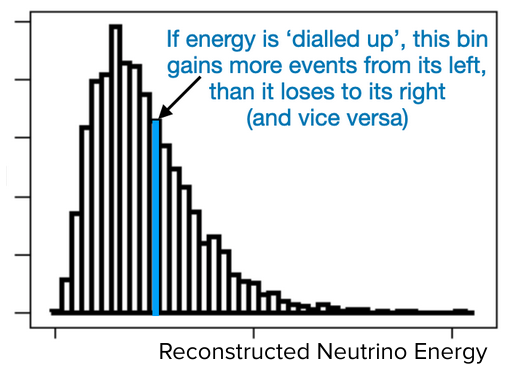
\includegraphics[width = \largefigwidth]{figures-chap5/energy_scale.png}
    \caption{Possible event migration due to uncertainty on the reconstructed neutrino energy.}
    \label{fig:energy_scale}
\end{figure}

Since the energy scale systematic is a global one, it is applied across all energy bins, for all modes, in the form a $1 \times 1$ covariance matrix.

\section{Other Analysis Choices}
All the stuff that was 'agreed' between fitters - Baseline Approximation, Binning, Spectra energy range etc.

\subsection{Baseline}
As is shown in \EquationRef{eqn:sterile_osc_prob}, the baseline is one of the components that drives the oscillation probability. For long baseline experiments, it's not uncommon for fitting frameworks to simply use some average value for the baseline since factors such as the interaction point in the detector or the position at which a particle decays into a neutrino would only change the average baseline for the experiment by a negligible amount. However, for short baseline experiments such as \gls{sbn}, these factors may change the baseline significantly. 

In an attempt to minimise computing resources, the true baseline was not initially used, but instead several approximations to the baseline were tried. To begin with, the average baseline of each \gls{sbn} detector was used for all neutrino energies. This was calculated from the true baseline distribution of \numu events in each detector which are shown in \FigureRef{fig:numu_baseline}. Secondly, a 4-knot spline (named spline V1) for each detector was defined in order to try and better approximate the baseline. This method was improved upon by producing a spline for each of the true energy bins (named spline V2) which are defined in \SectionRef{sec:binning}. In order to establish the impact of any baseline approximations on the oscillation probability, the oscillation probability was plotted as a function of true neutrino energy with the oscillation parameters $sin^22\theta_{\mu\mu} = 0.01$ and $\Delta m^2_{41} = 50$ eV$^2$. This oscillation point was chosen to ensure that a region where rapid oscillation occur was being investigated, which would highlight the effect of any baseline choices. The oscillation probabilities as a function of energy are shown in \FigureRef{fig:baseline_osc_probability} for the four different baselines described. It was eventually decided that any approximation would be insufficient and that the true baseline should be used. 

The studies of the baseline approximations were done in the context of the \numu disappearance channel. For the \nue channels, different approximations should be applied, since the true baseline distribution is not the same as for \numu. In principal, within the \nue sample, different approximations should be applied to the different sub-samples since the baseline distribution is not the same for all the sub-samples. This was never done since it was decided that the true baseline should be used. Each individual sample used to construct the overall \nue event sample, has it's own baseline distribution due to the particles which contribute to each sample decaying at different points along the beamline. The baseline distribution for the intrinsic \nue, oscillated \nue and the overall \nue sample from combining all the sub-samples together is shown in \FigureRef{fig:nue_baseline_dist} for each of the \gls{sbn} detectors. It should be noted that the baseline distributions for oscillated \nue sample from \FigureRef{fig:nue_baseline_dist} and the \numu sample from \FigureRef{fig:numu_baseline} are comparable. This is due to the initial parameters describing the oscillated sample being the same as for the \numu sample. The only difference being the neutrino oscillations from \numu to \nue which isn't something that affects the baseline.

\begin{figure}[!h]
    \centering
    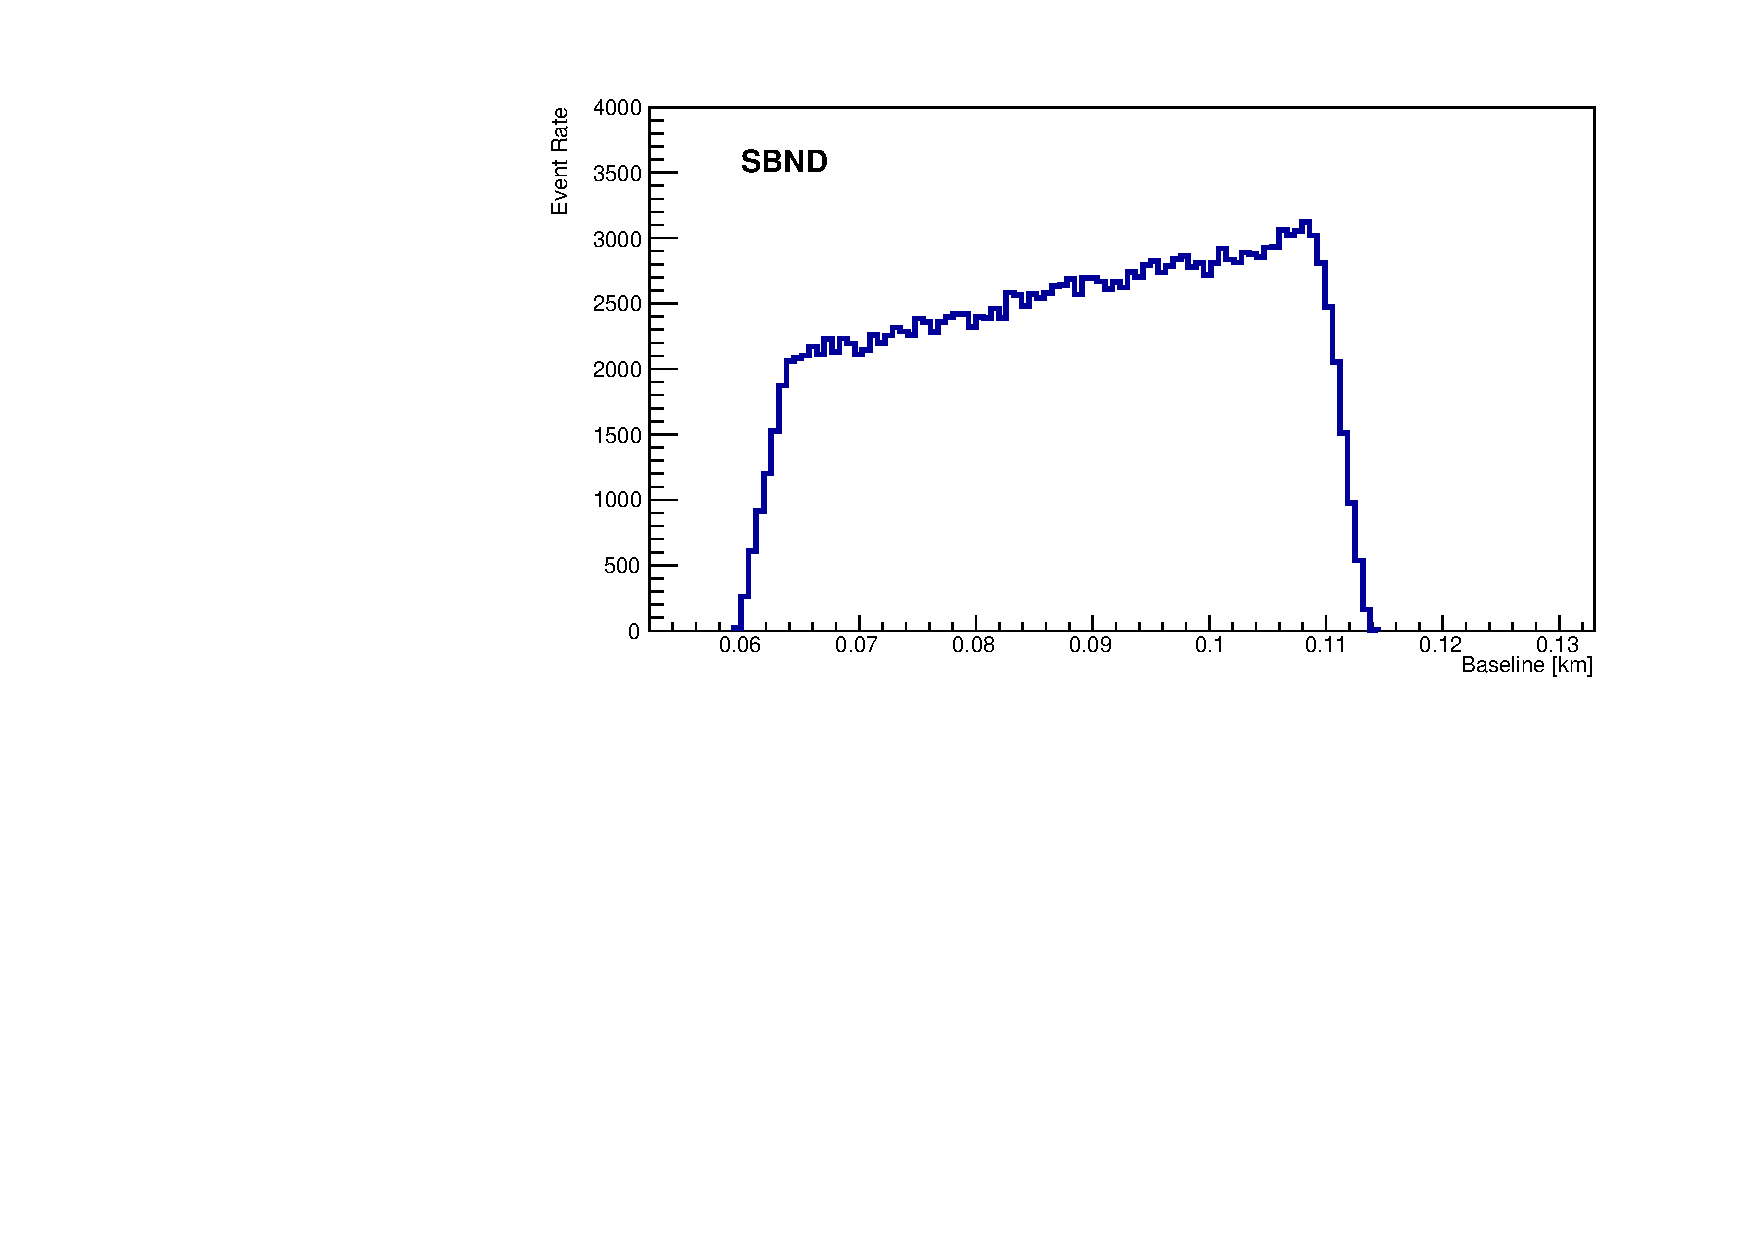
\includegraphics[width = 0.32\textwidth]{figures-chap5/SBND_numu.pdf}
    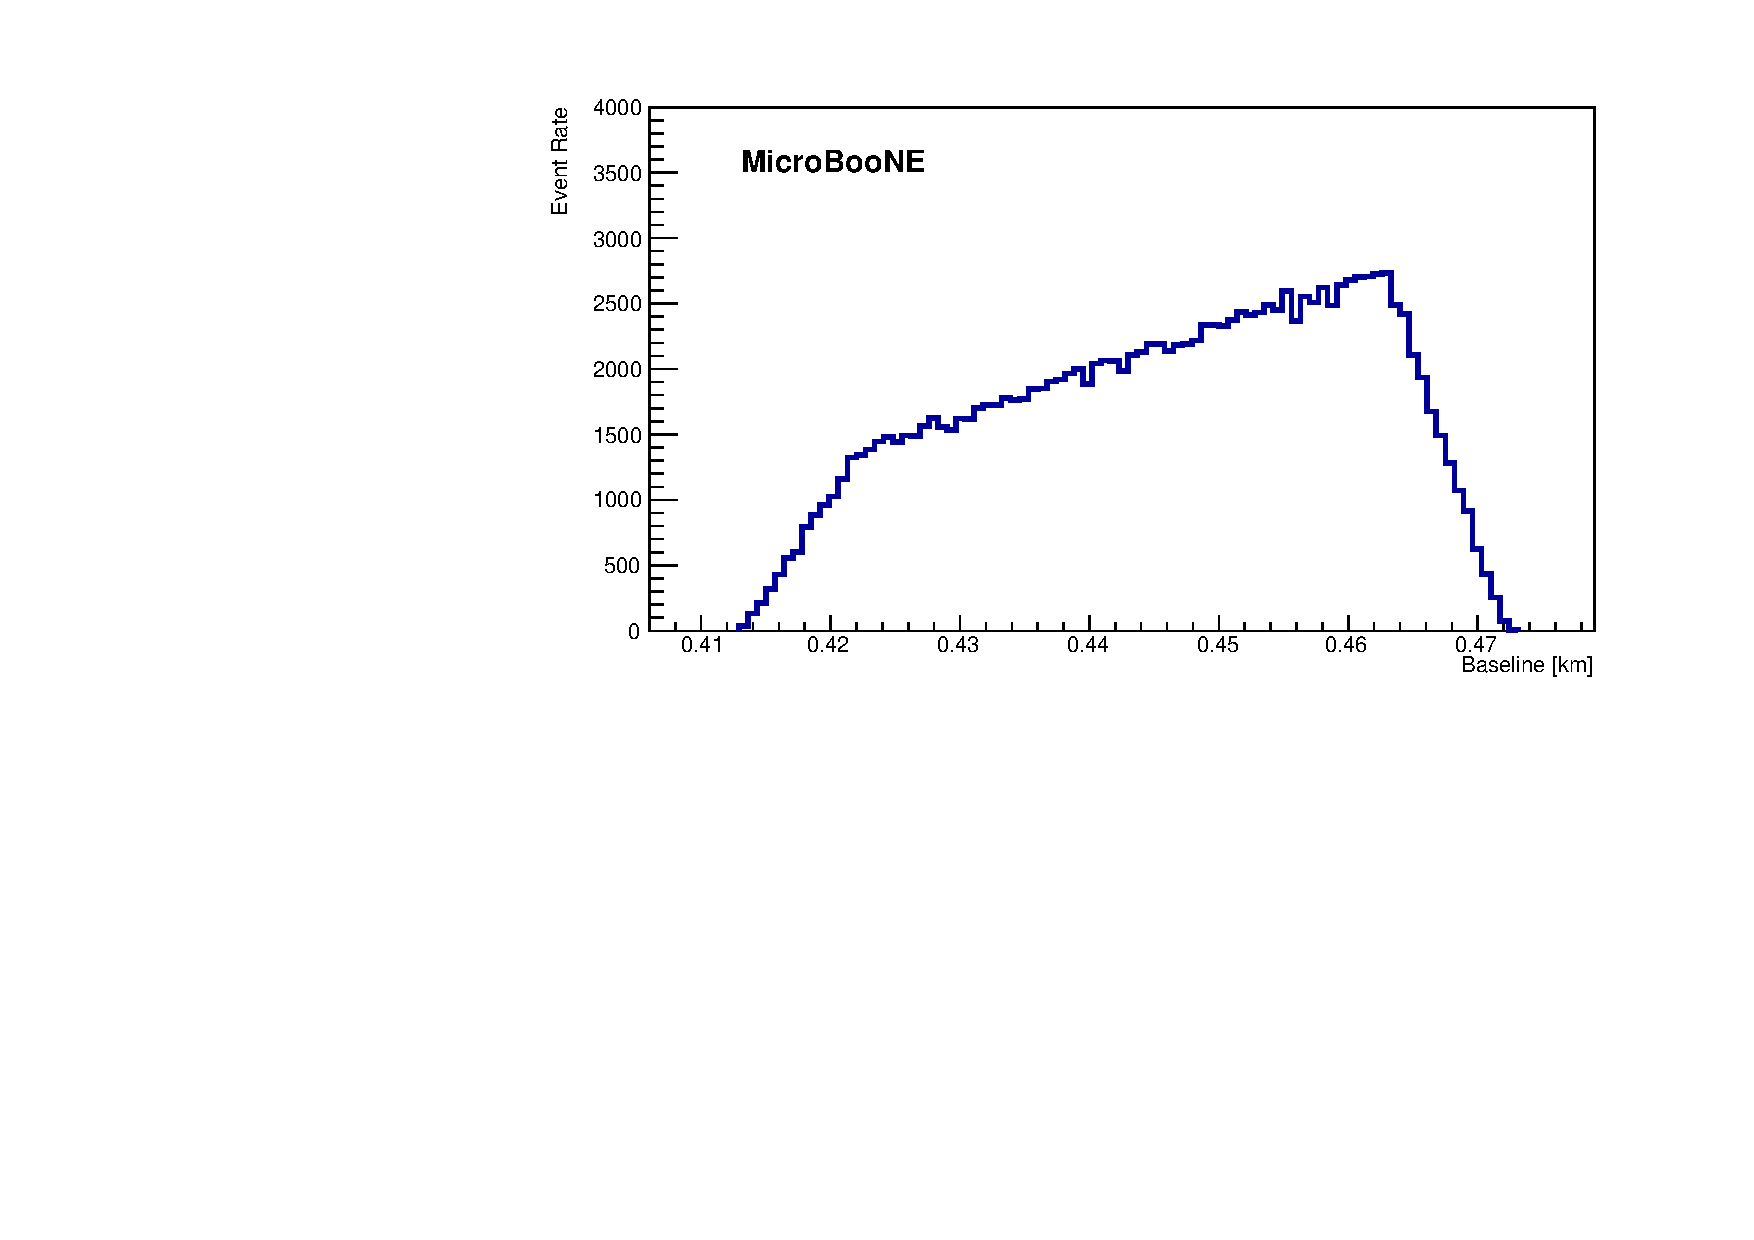
\includegraphics[width = 0.32\textwidth]{figures-chap5/MicroBooNE_numu.pdf}
    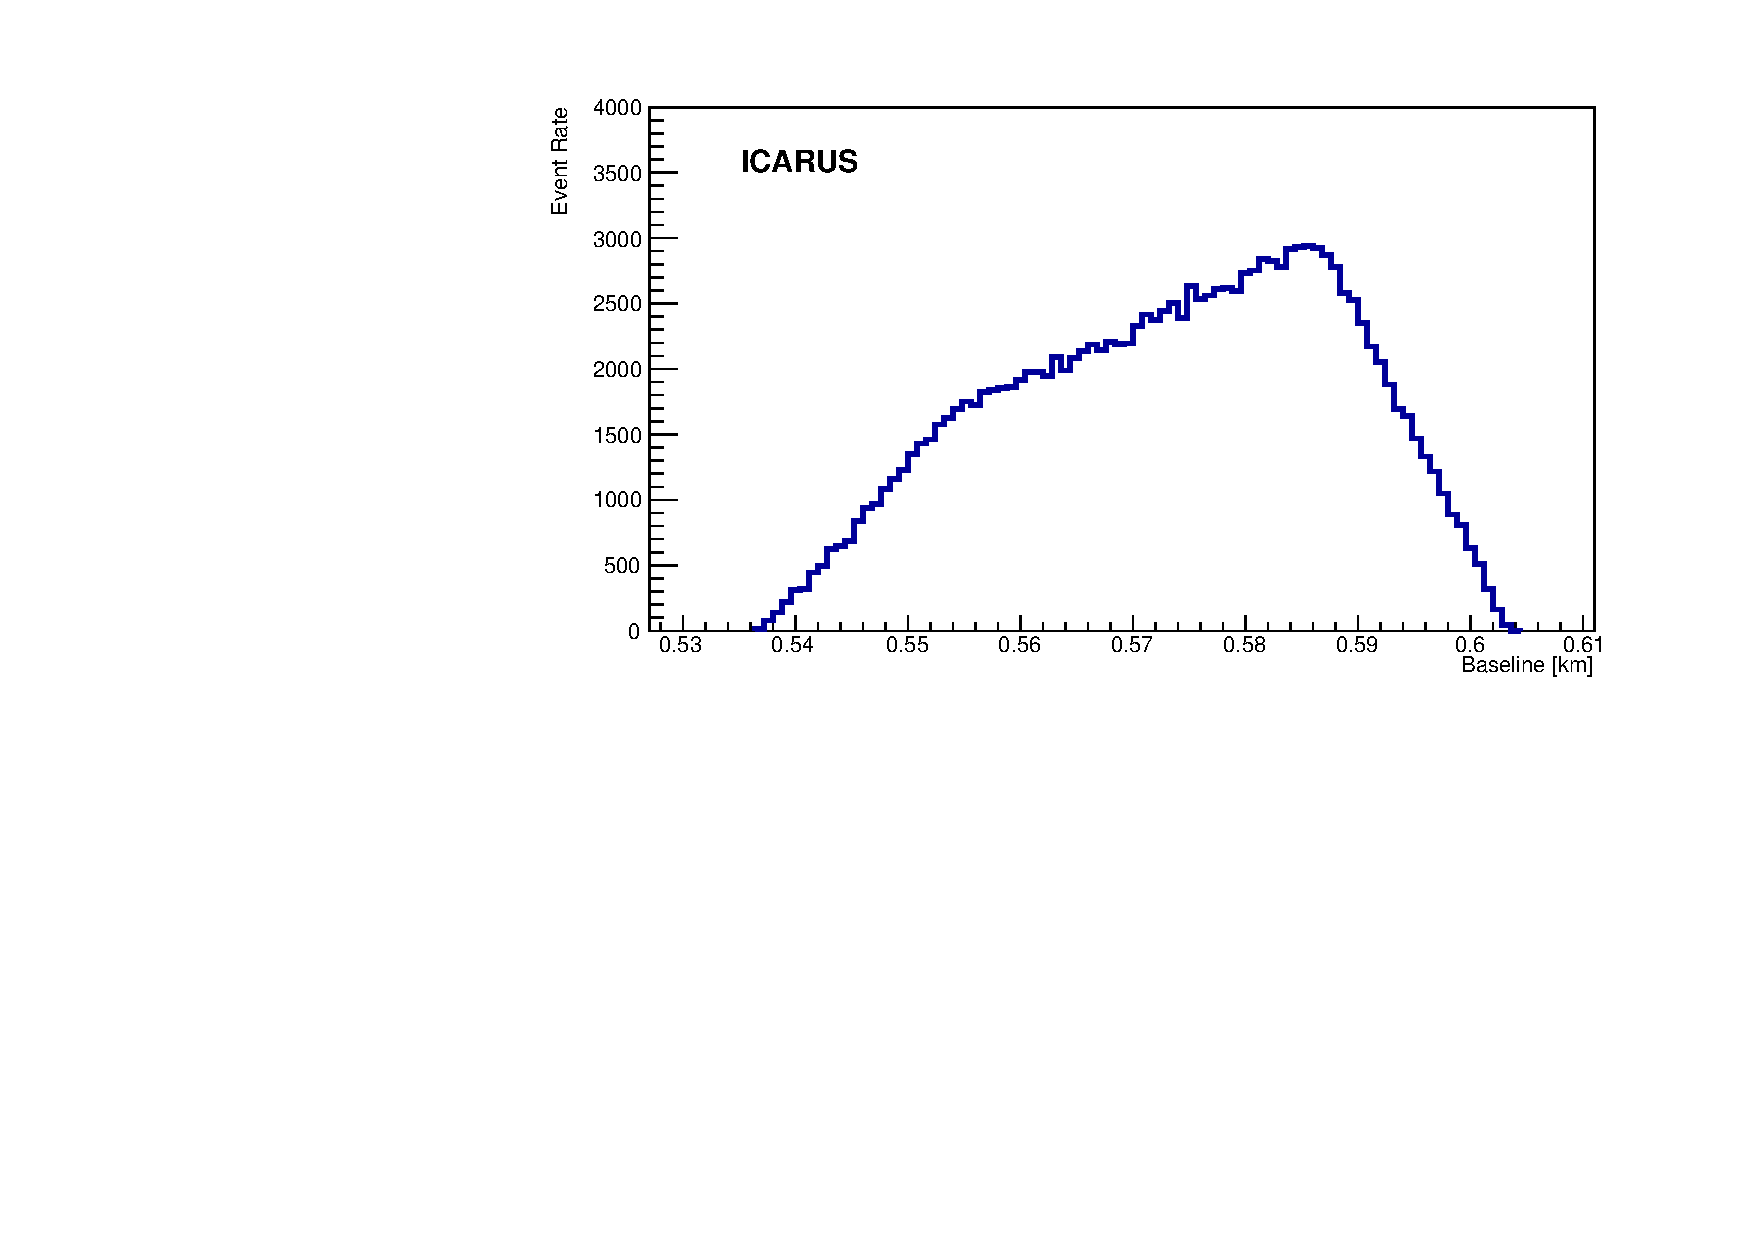
\includegraphics[width = 0.32\textwidth]{figures-chap5/ICARUS_numu.pdf}
    \caption{The baseline distribution of events in the \numu sample for each of the \gls{sbn} detectors.}
    \label{fig:numu_baseline}
\end{figure}

\begin{figure}[!h]
    \centering
    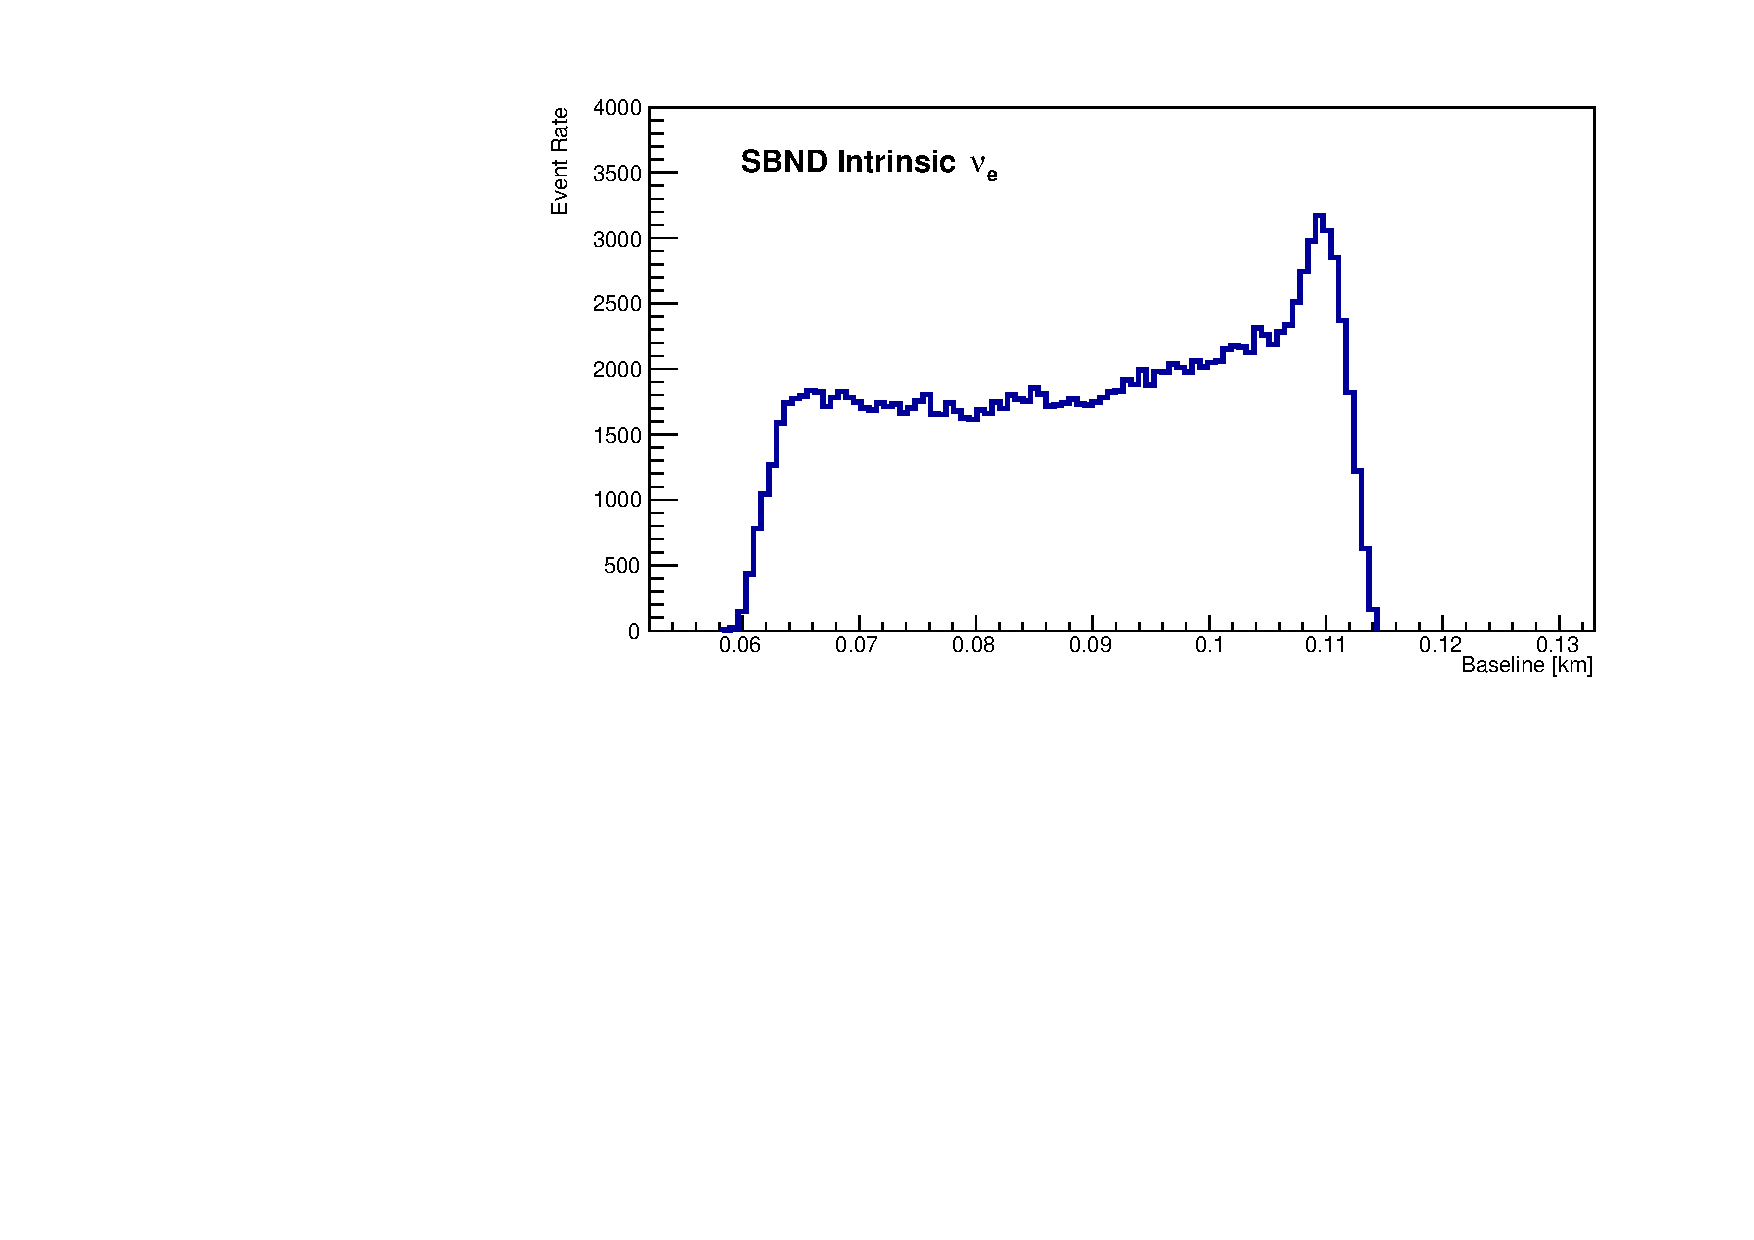
\includegraphics[width = 0.32\textwidth]{figures-chap5/SBND_intrinsic_nue.pdf}
    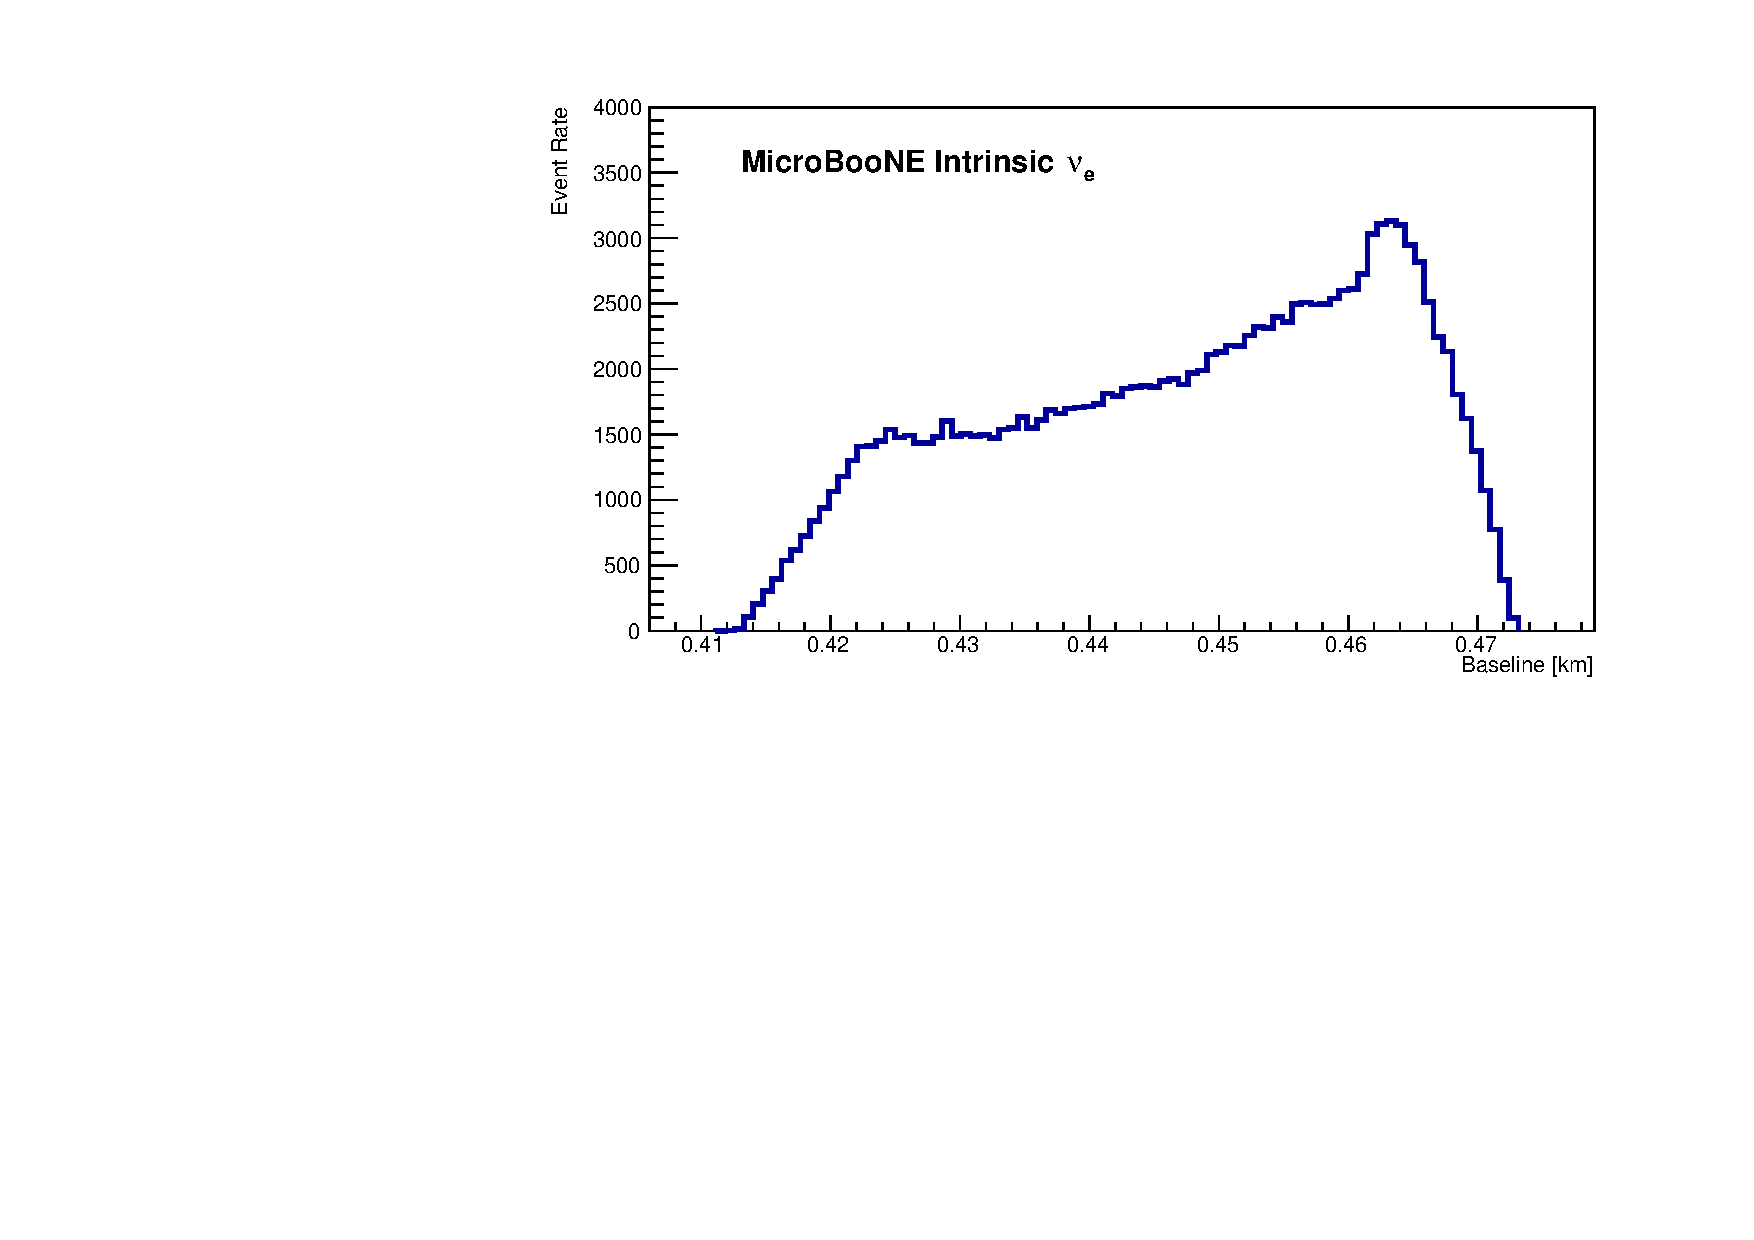
\includegraphics[width = 0.32\textwidth]{figures-chap5/MicroBooNE_intrinsic_nue.pdf}
    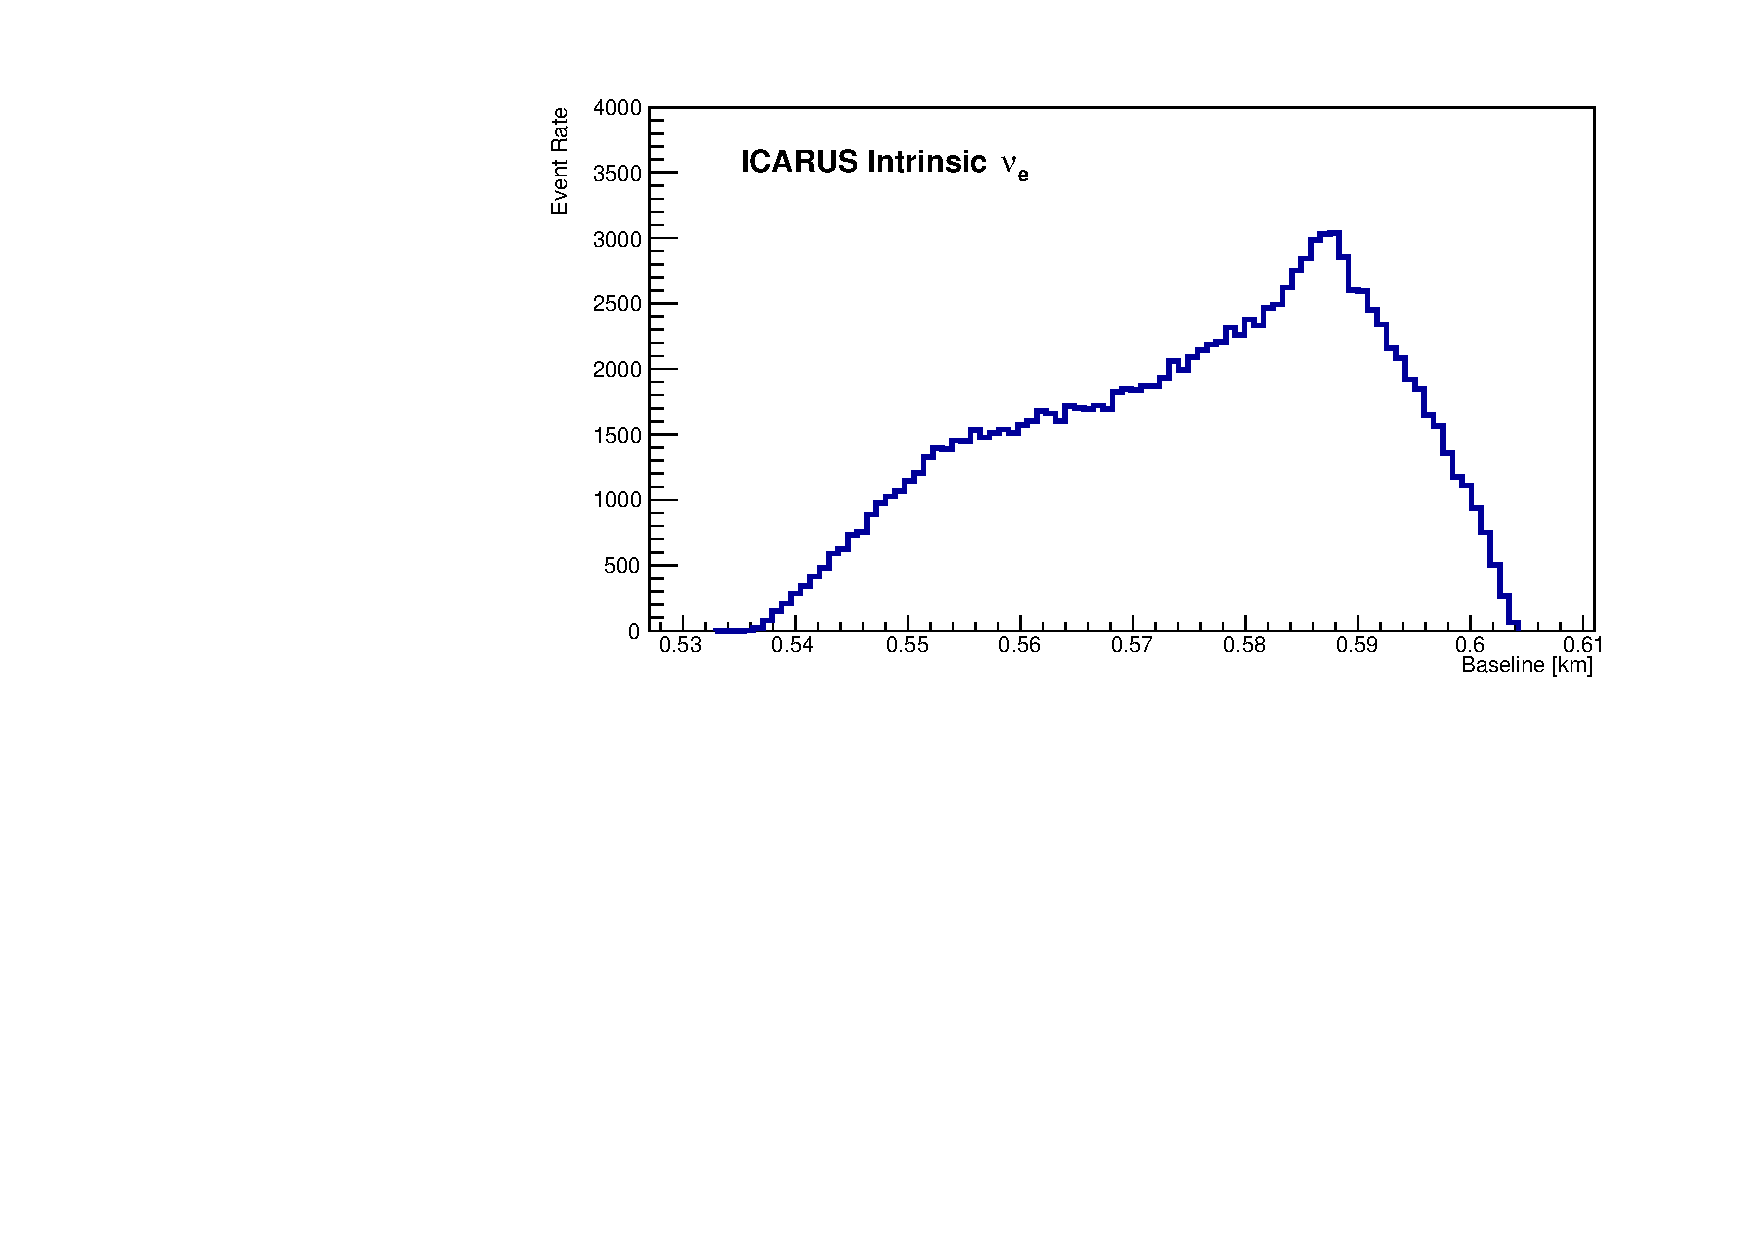
\includegraphics[width = 0.32\textwidth]{figures-chap5/ICARUS_intrinsic_nue.pdf} 
    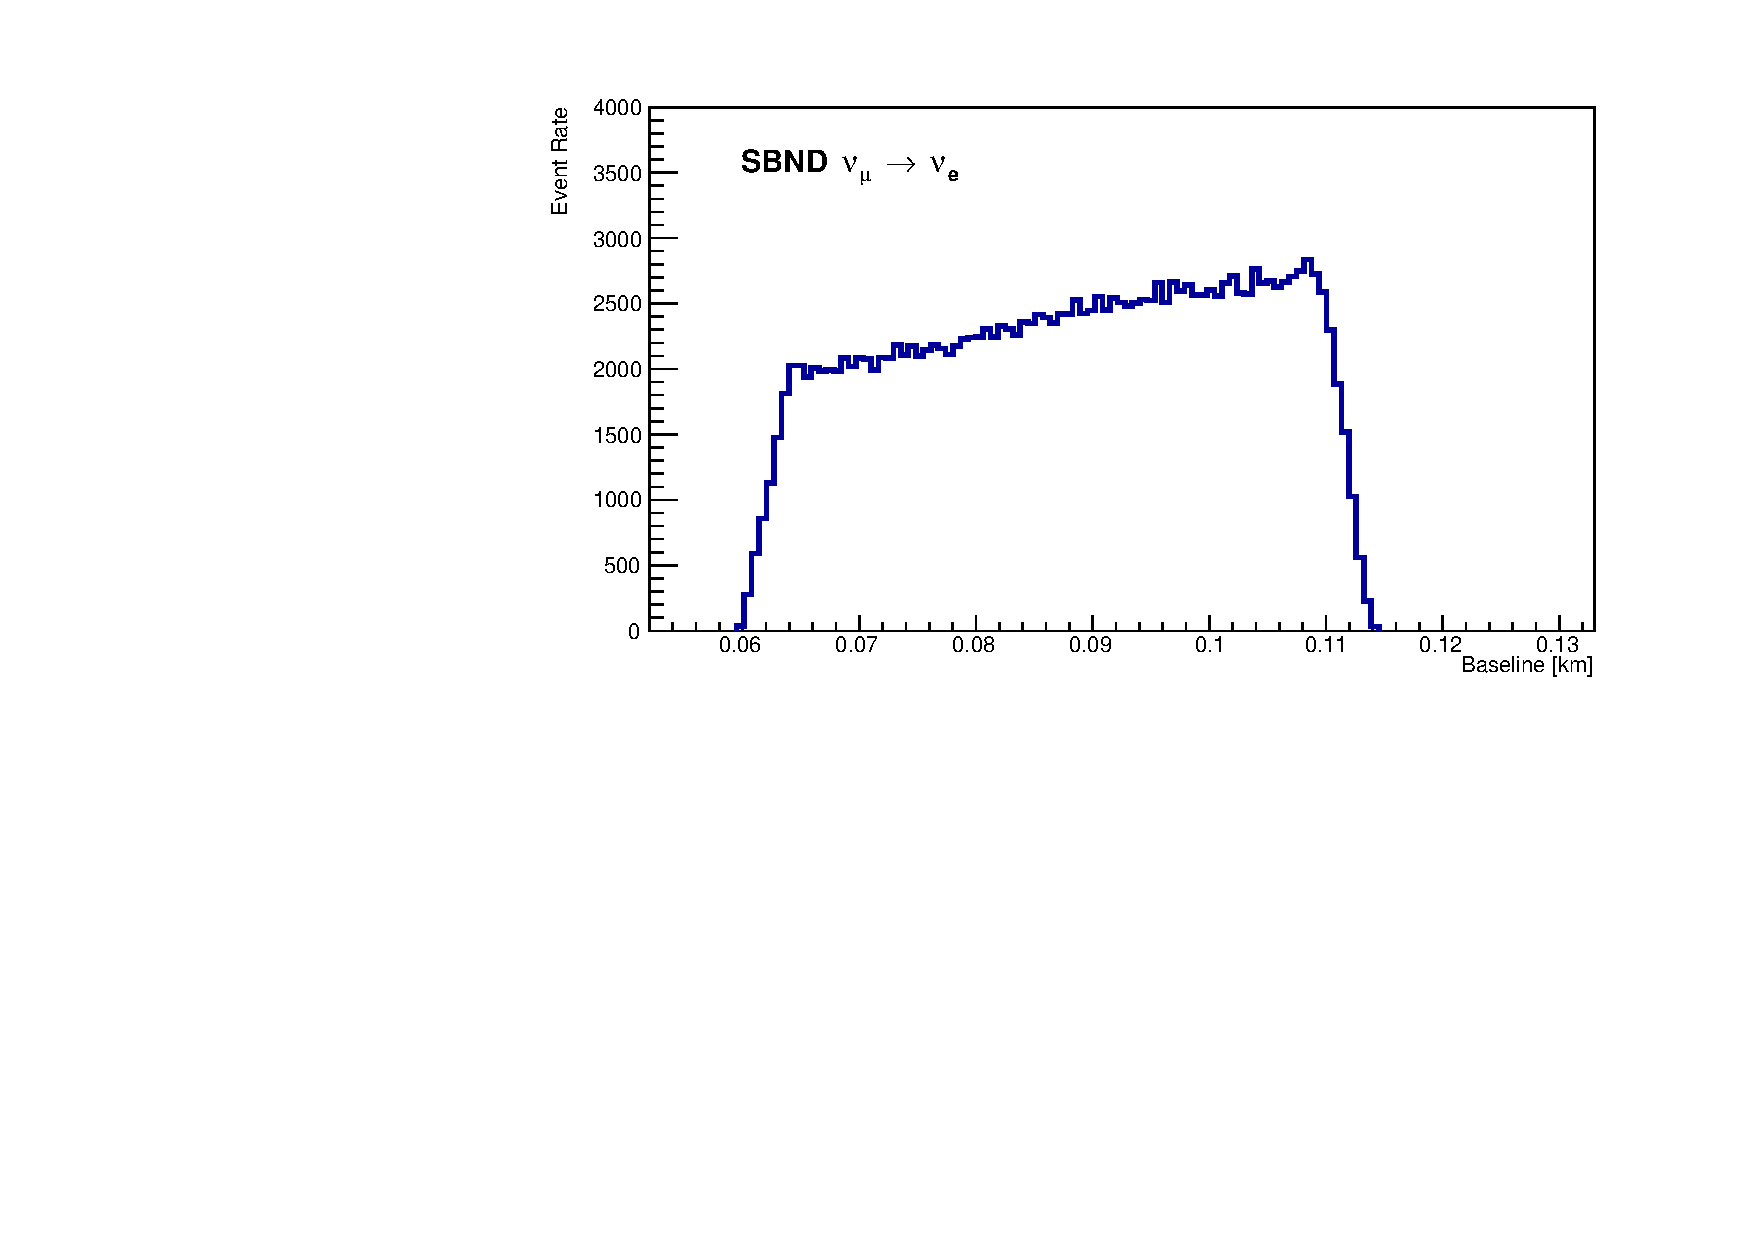
\includegraphics[width = 0.32\textwidth]{figures-chap5/SBND_osc.pdf}
    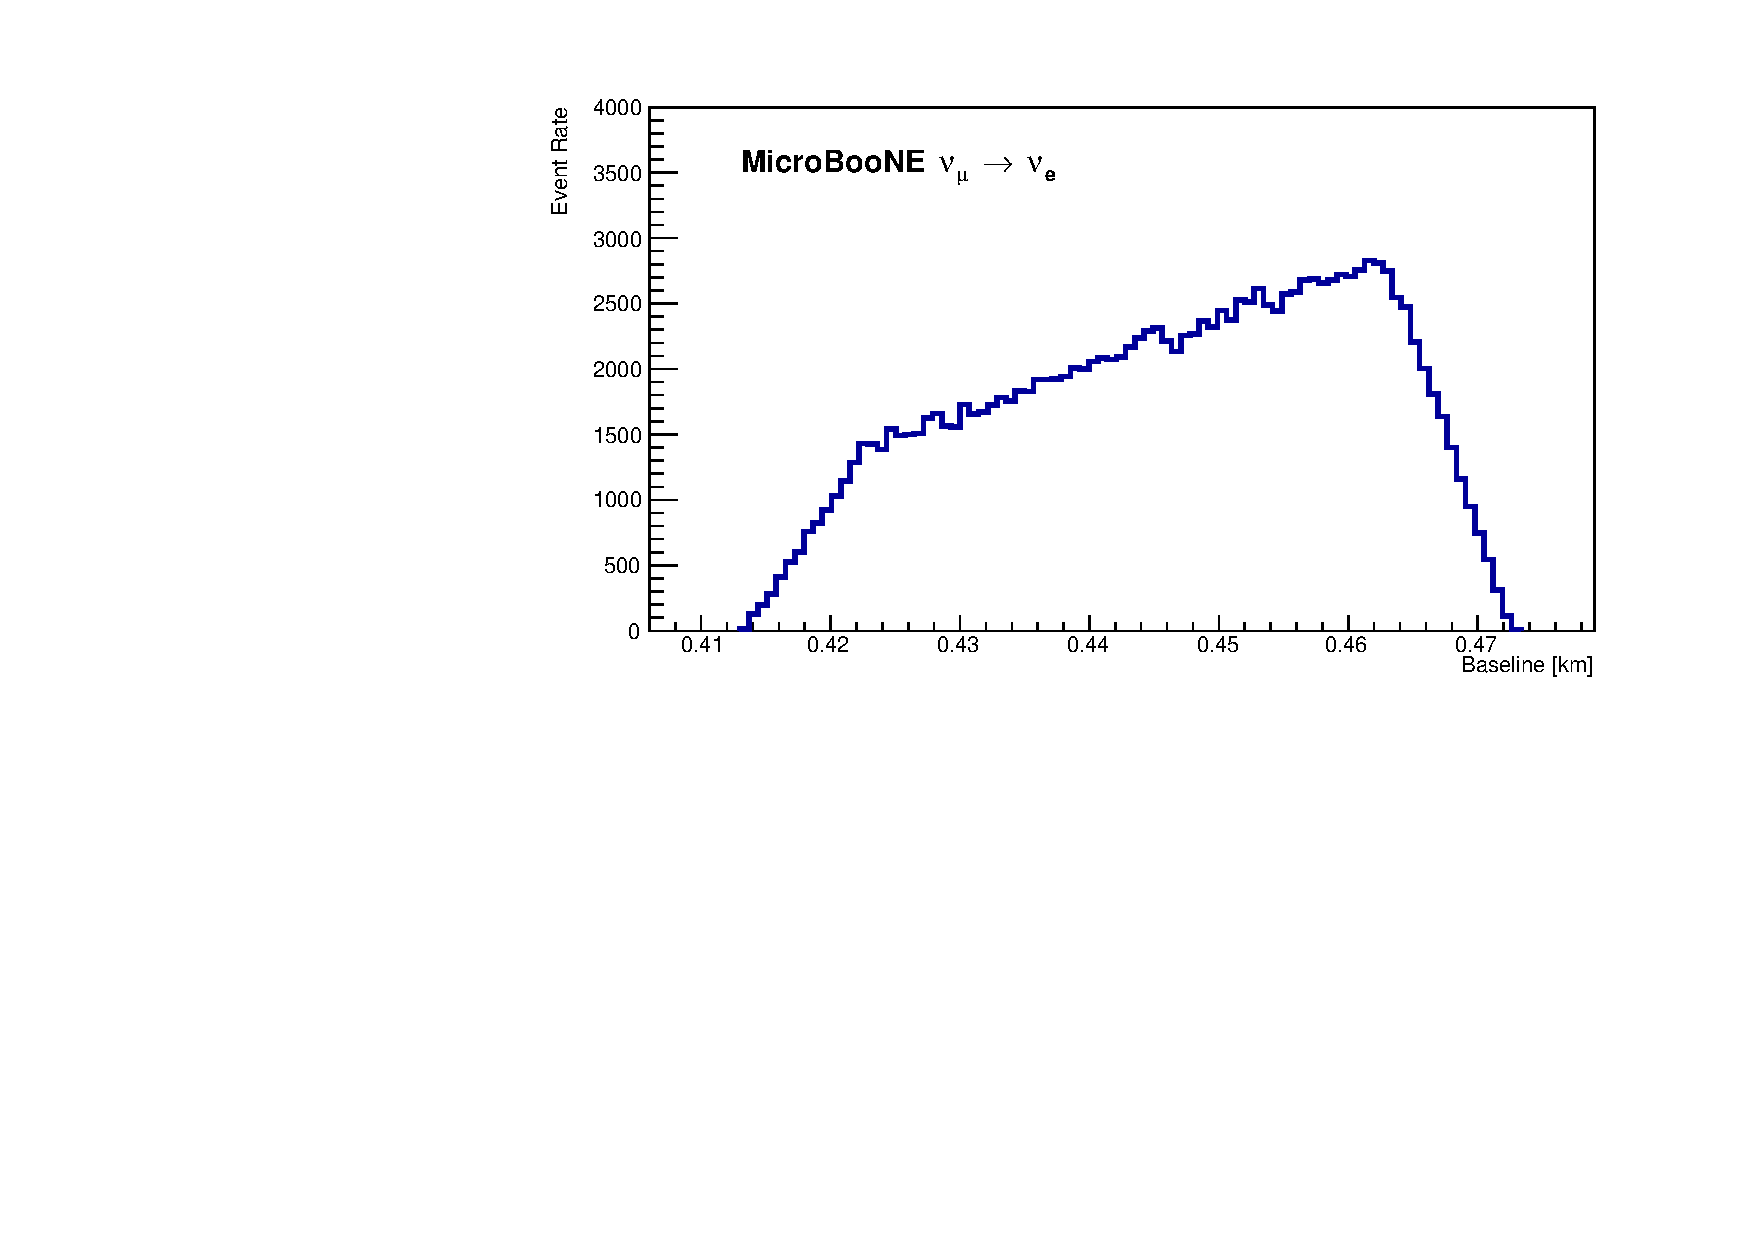
\includegraphics[width = 0.32\textwidth]{figures-chap5/MicroBooNE_osc.pdf}
    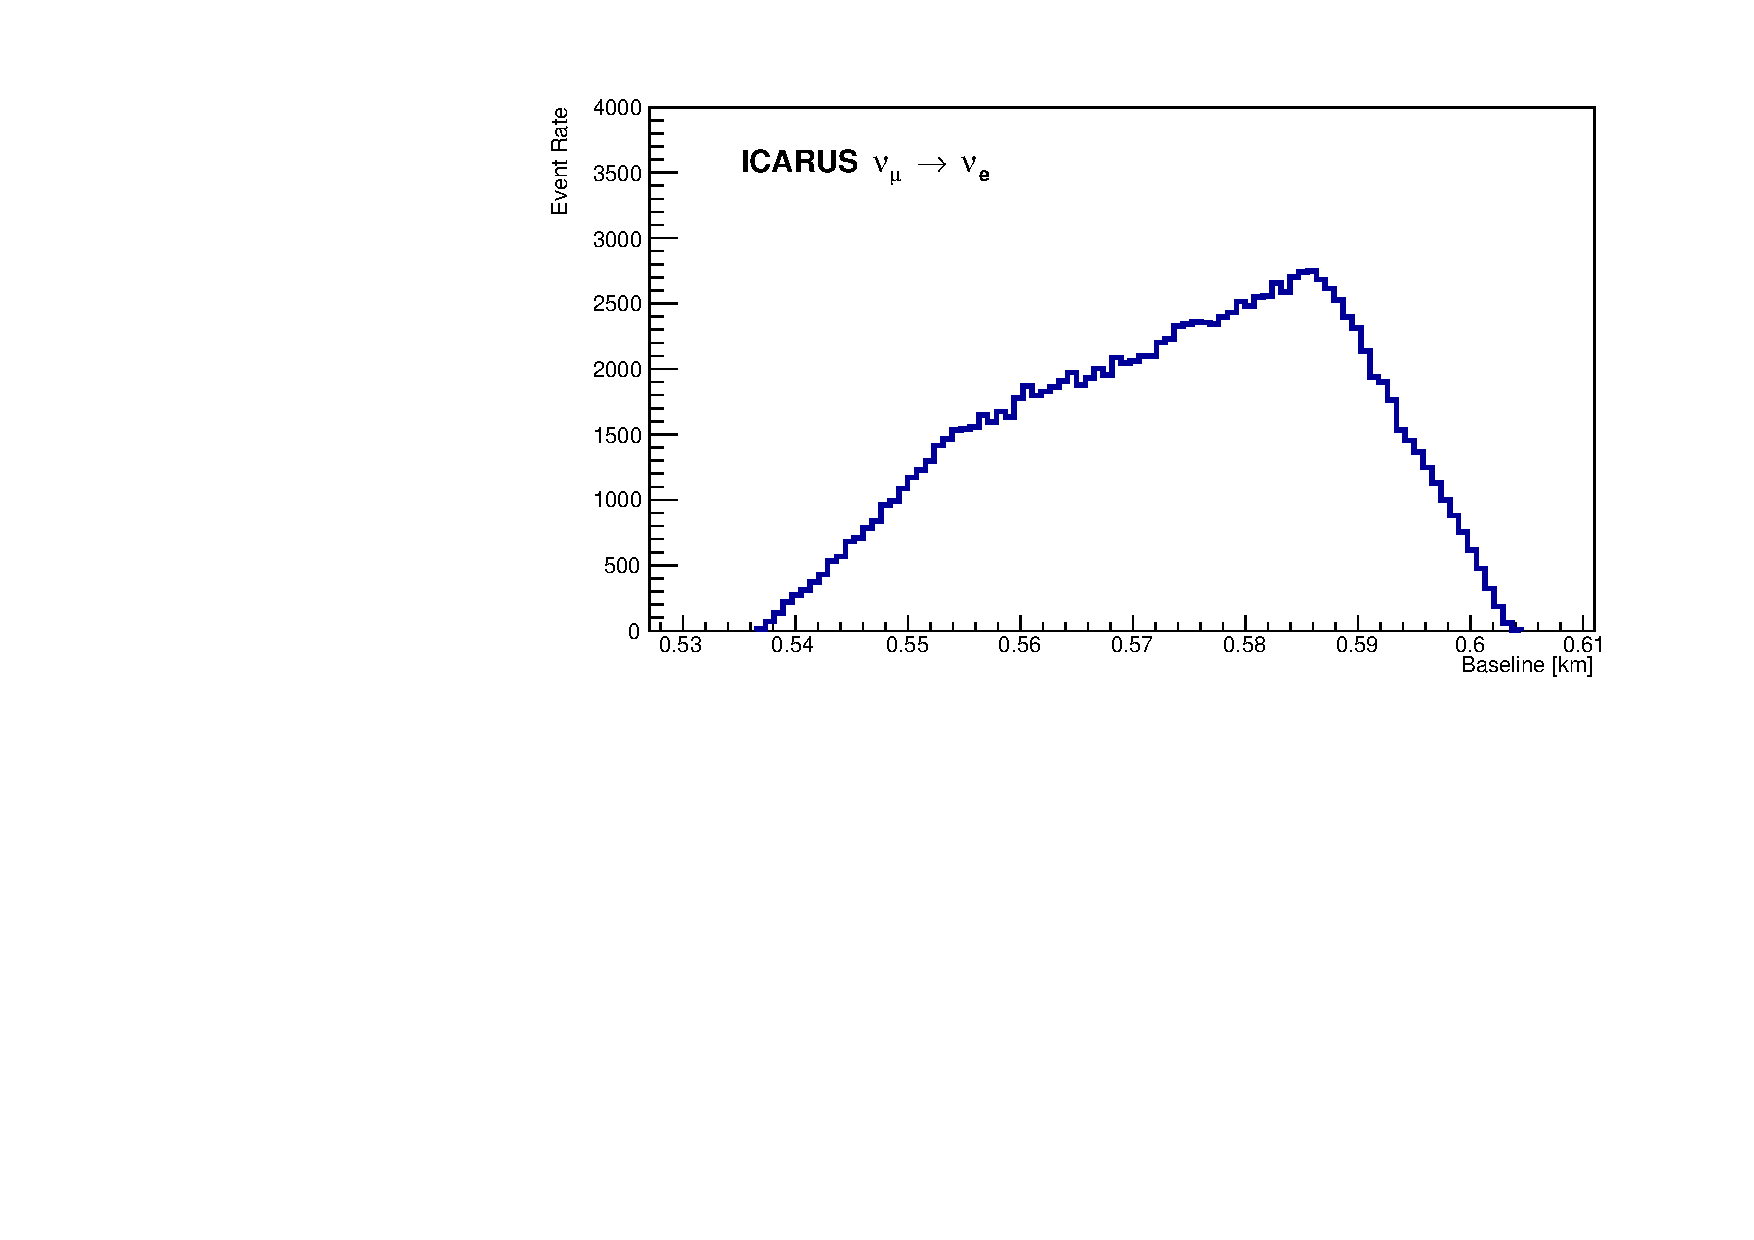
\includegraphics[width = 0.32\textwidth]{figures-chap5/ICARUS_osc.pdf}
    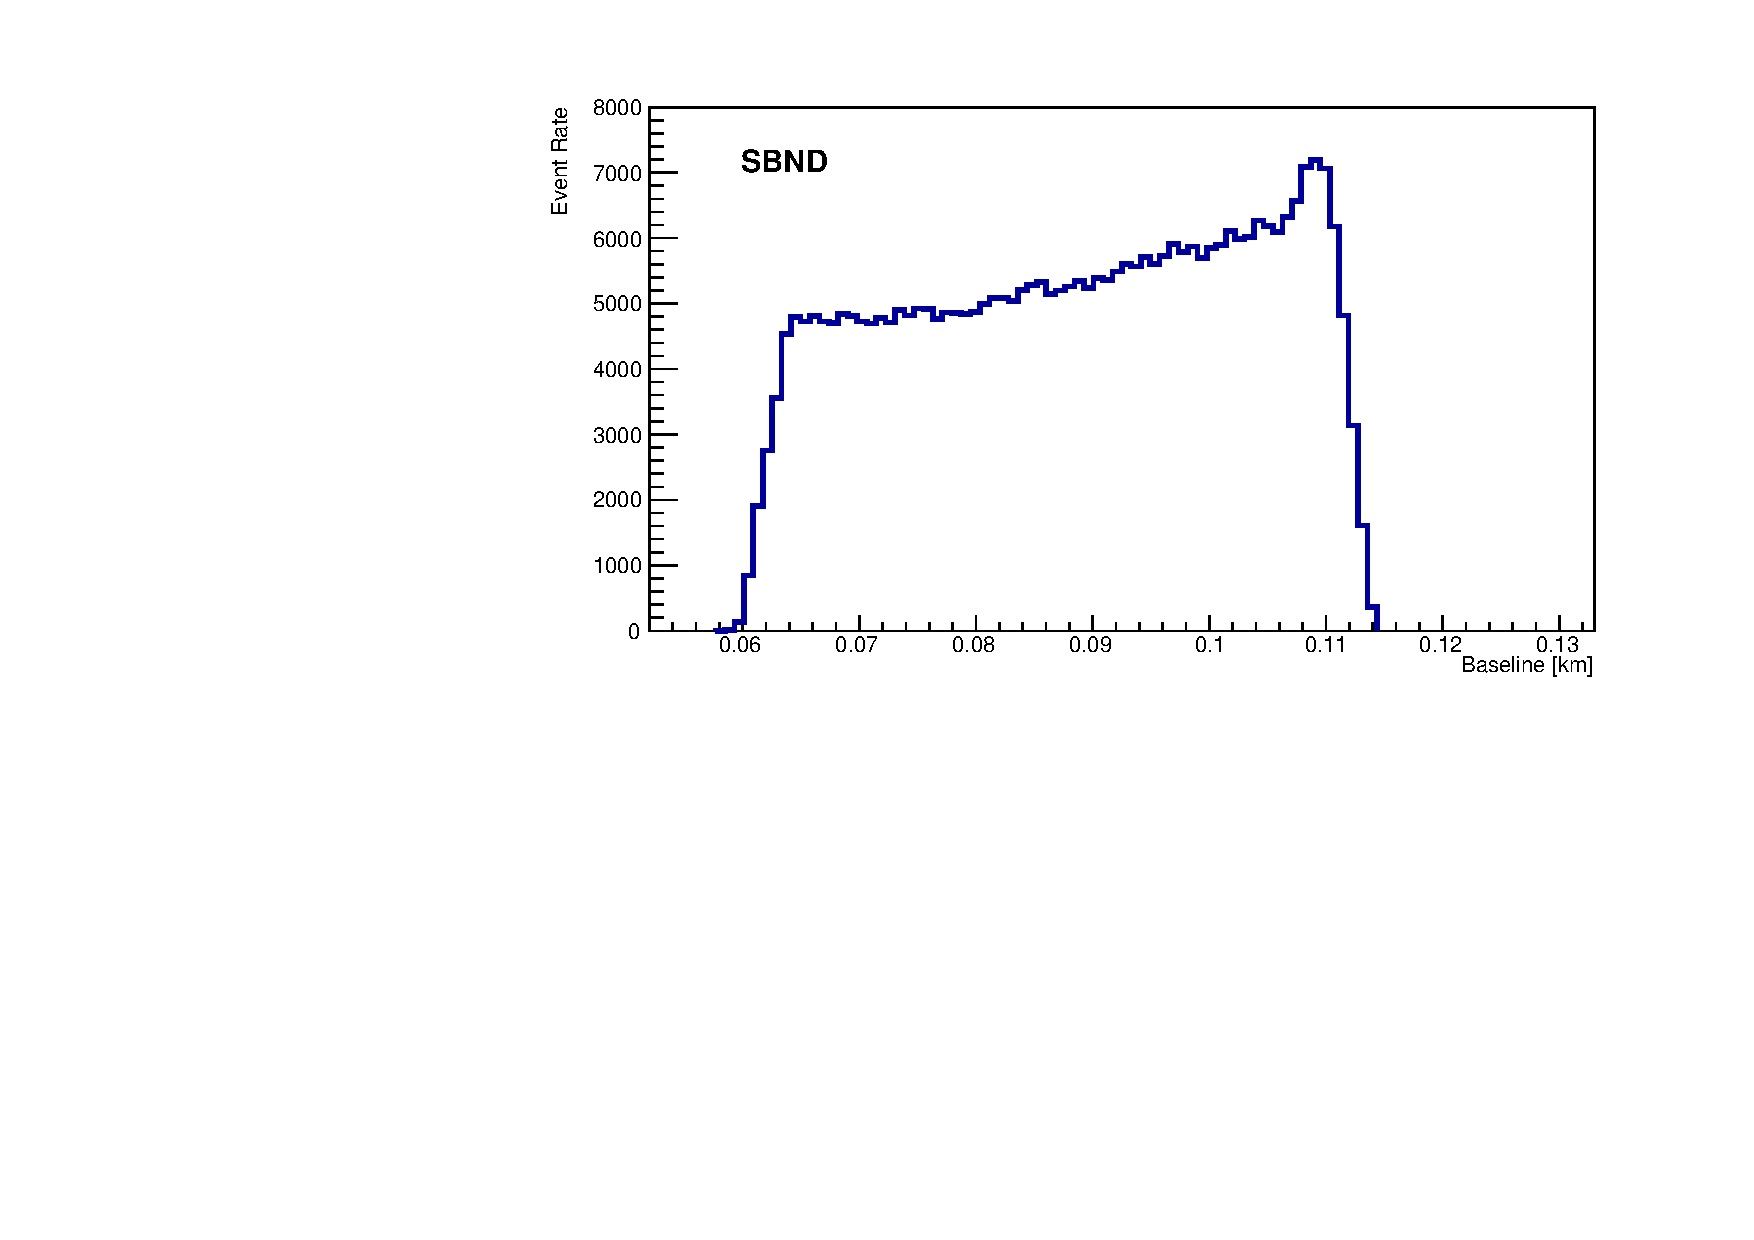
\includegraphics[width = 0.32\textwidth]{figures-chap5/SBND_nue.pdf}
    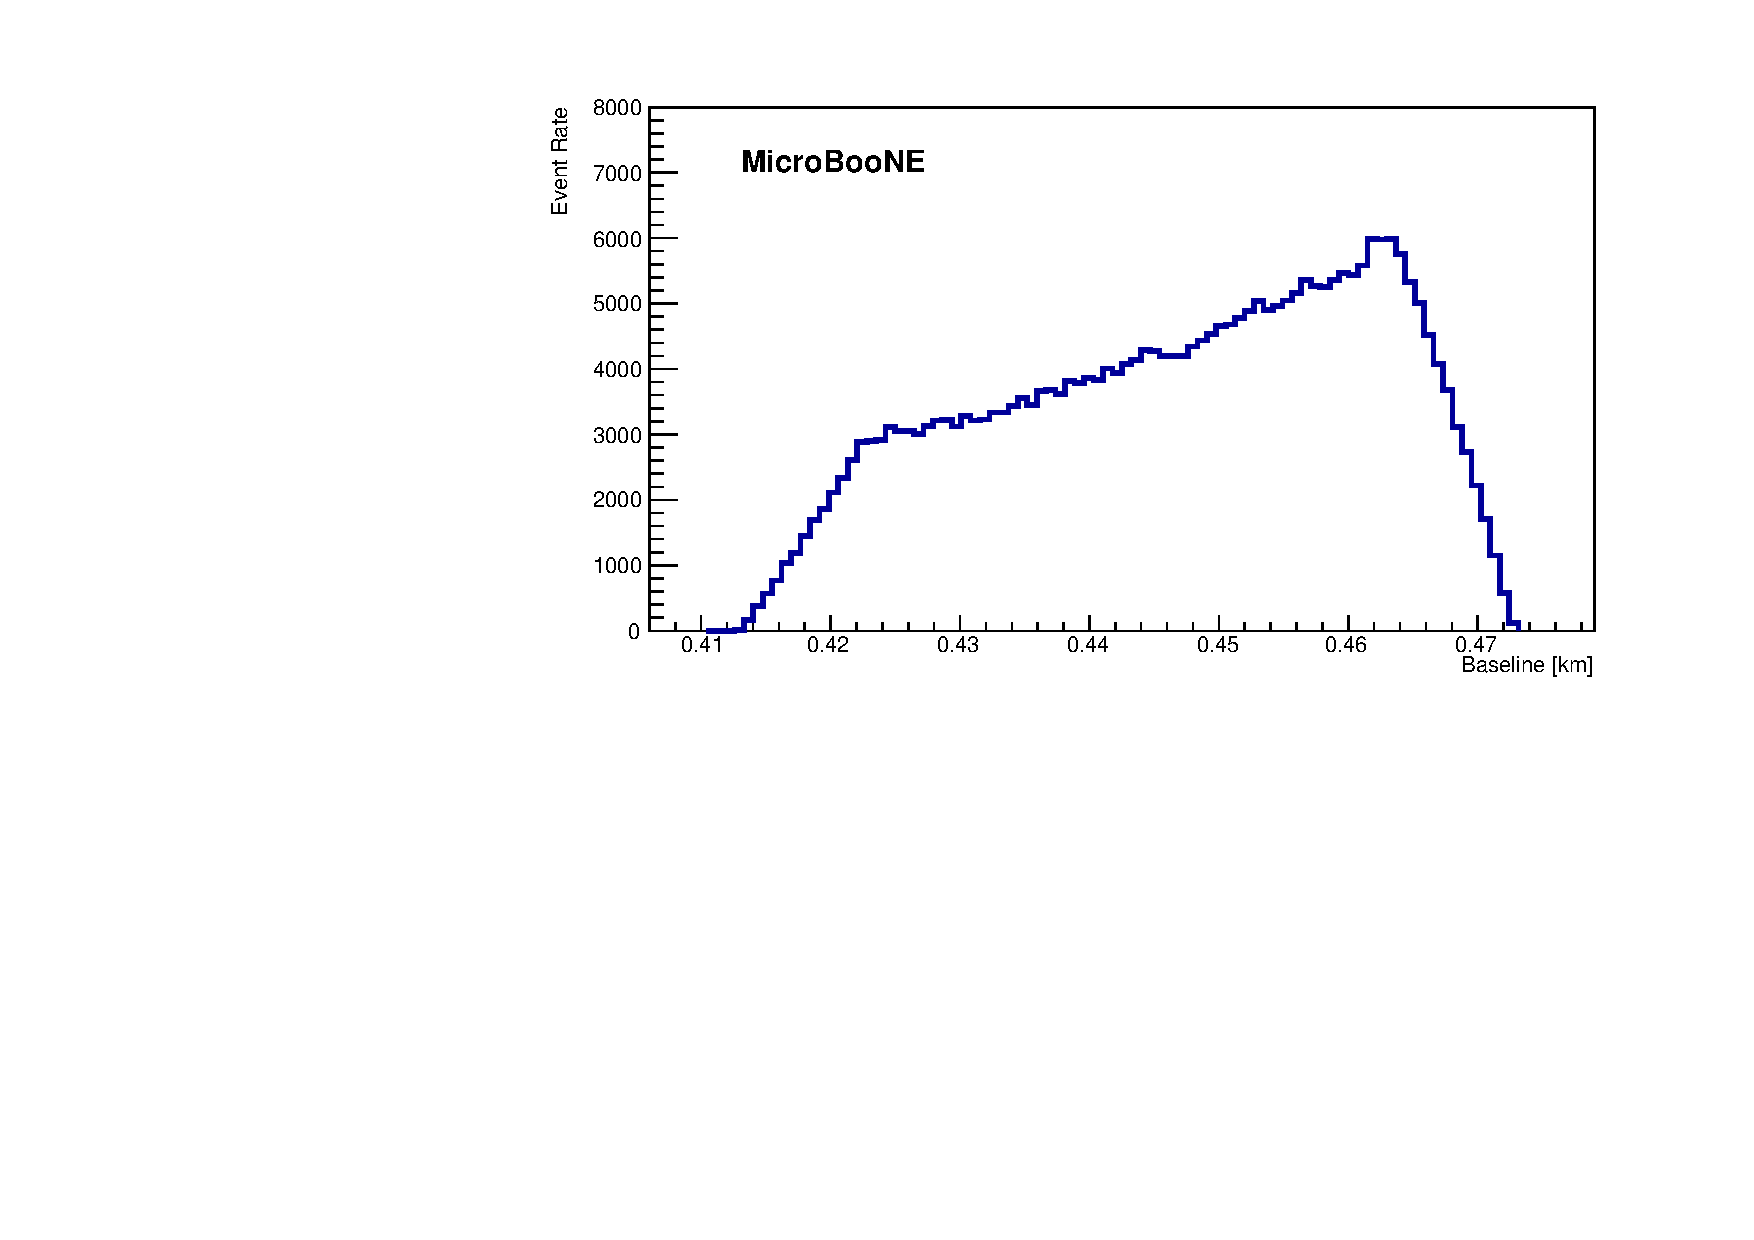
\includegraphics[width = 0.32\textwidth]{figures-chap5/MicroBooNE_nue.pdf}
    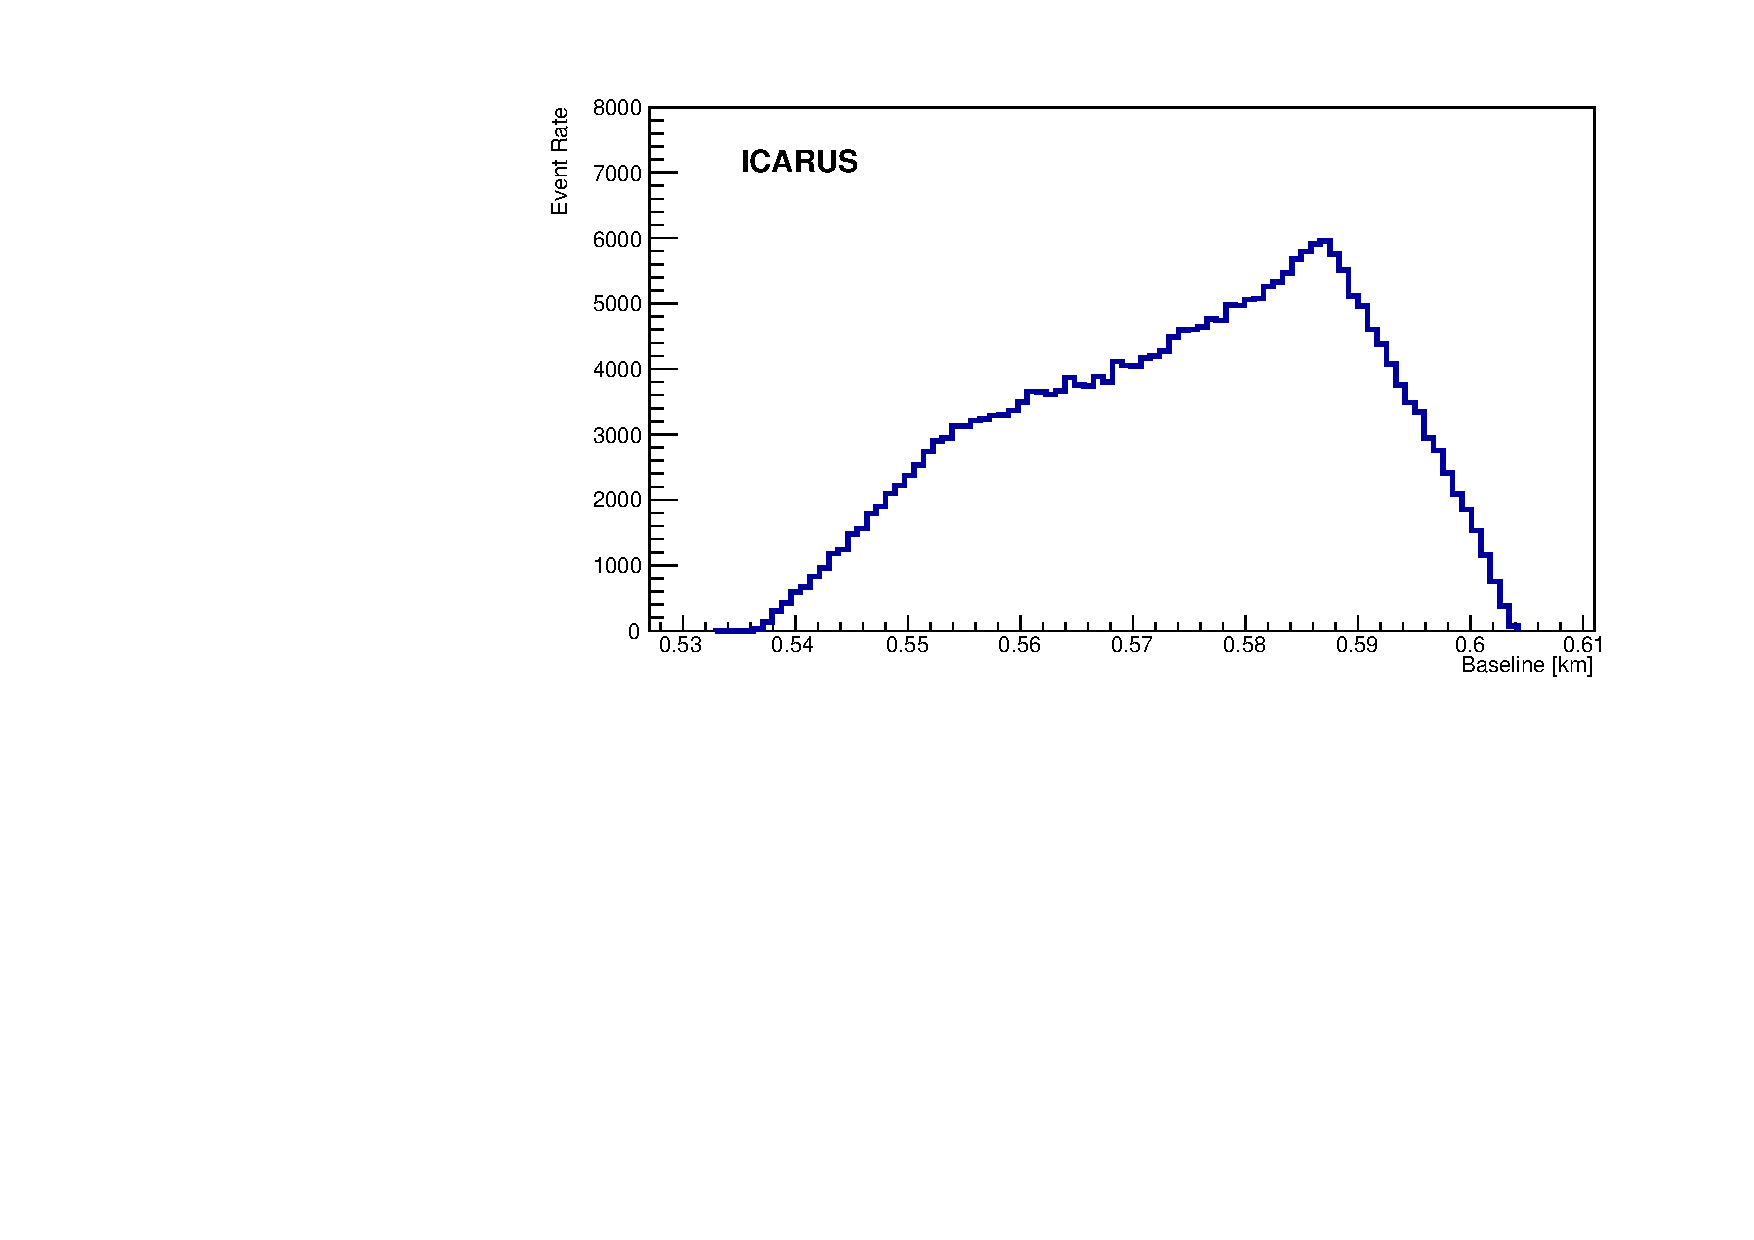
\includegraphics[width = 0.32\textwidth]{figures-chap5/ICARUS_nue.pdf}
    \caption{The baseline distribution of events in each of the \gls{sbn} detectors for the intrinsic \nue sample (Top), the oscillated \nue sample (Middle) and the overall \nue sample (Bottom). The overall sample is comprised of the events from the intrinsic \nue, oscillated \nue, the \numu events from \FigureRef{fig:numu_baseline} passing the \nue selection and the dirt and cosmic samples (which are not explicitly shown).
    The overall baseline distribution for events used in the \nue sample in each of the three \gls{sbn} detectors.}
    \label{fig:nue_baseline_dist}
\end{figure}

\begin{figure}[!h]
    \centering
    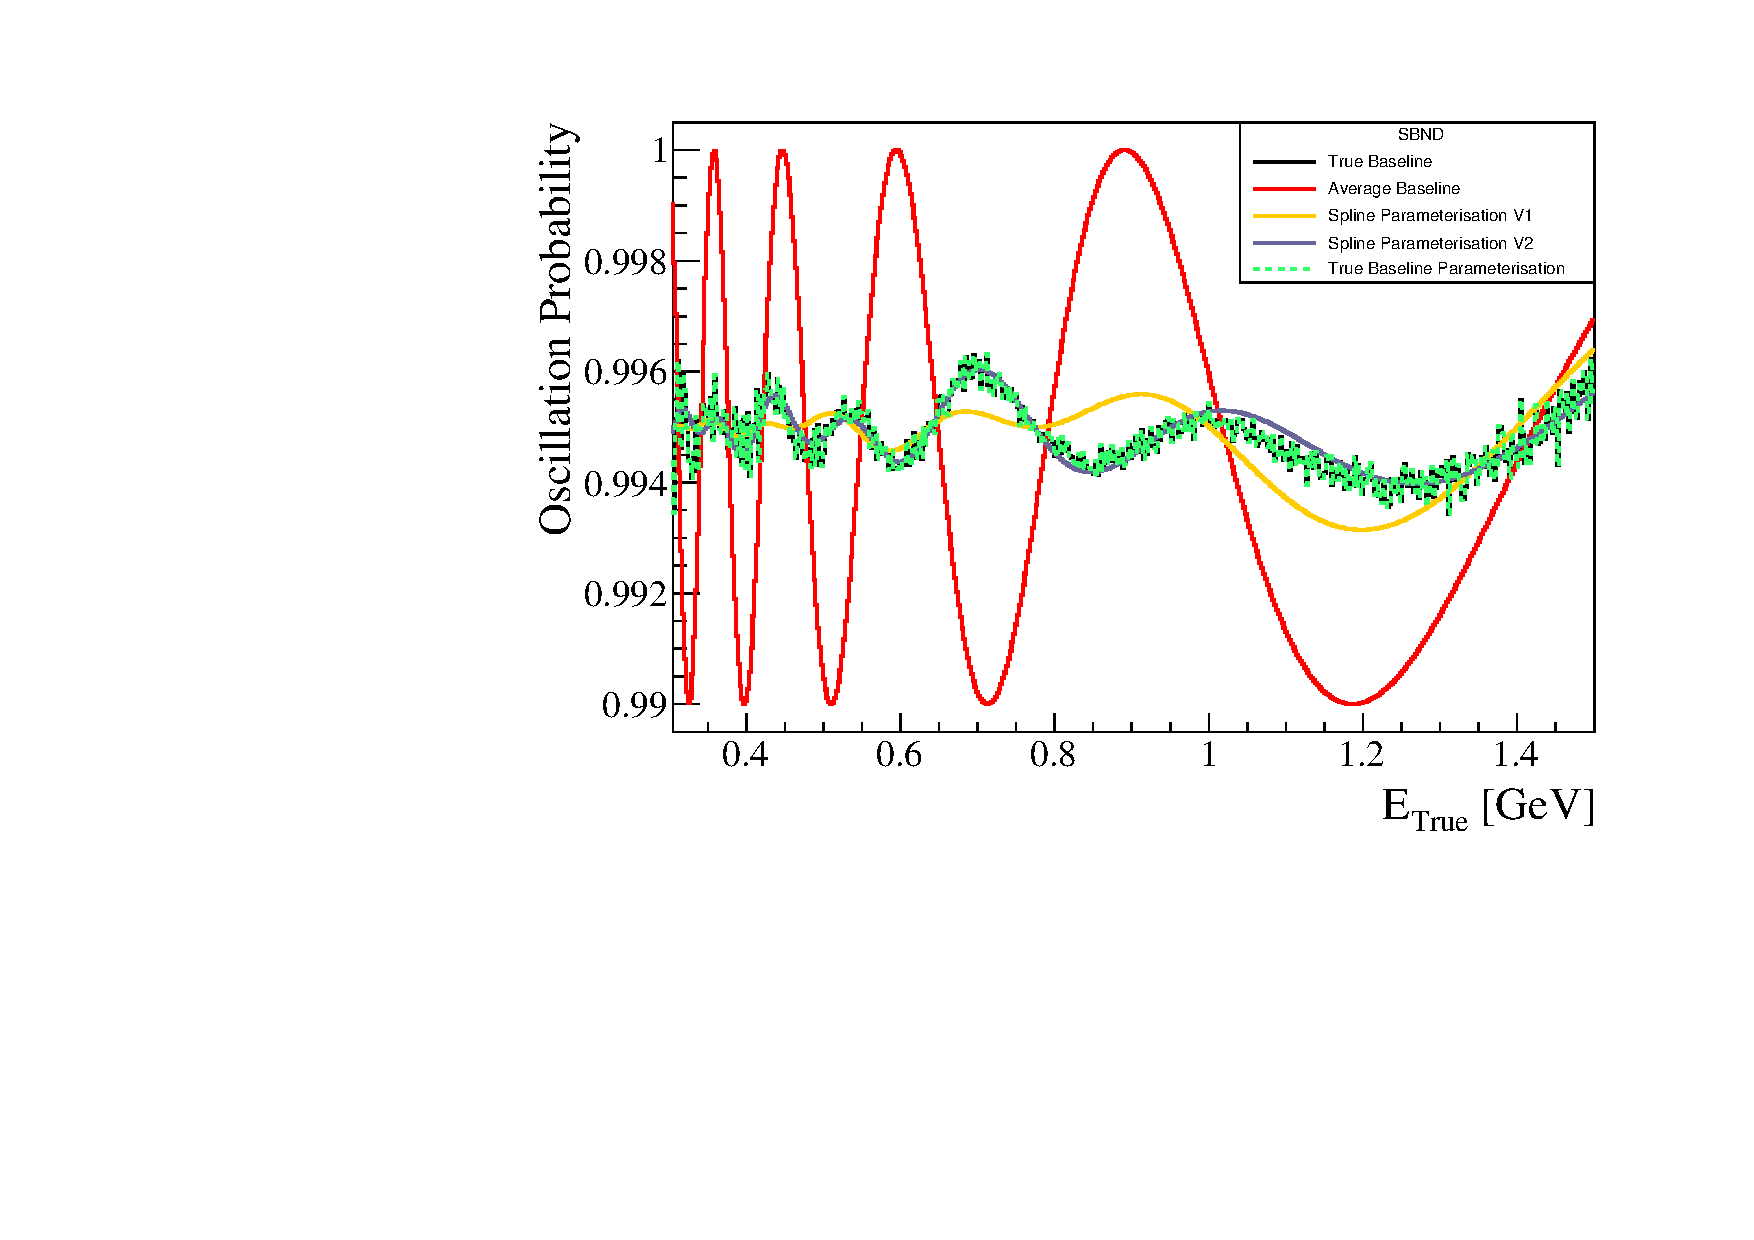
\includegraphics[width = 0.32\textwidth]{figures-chap5/osc_prob_sbnd.pdf}
    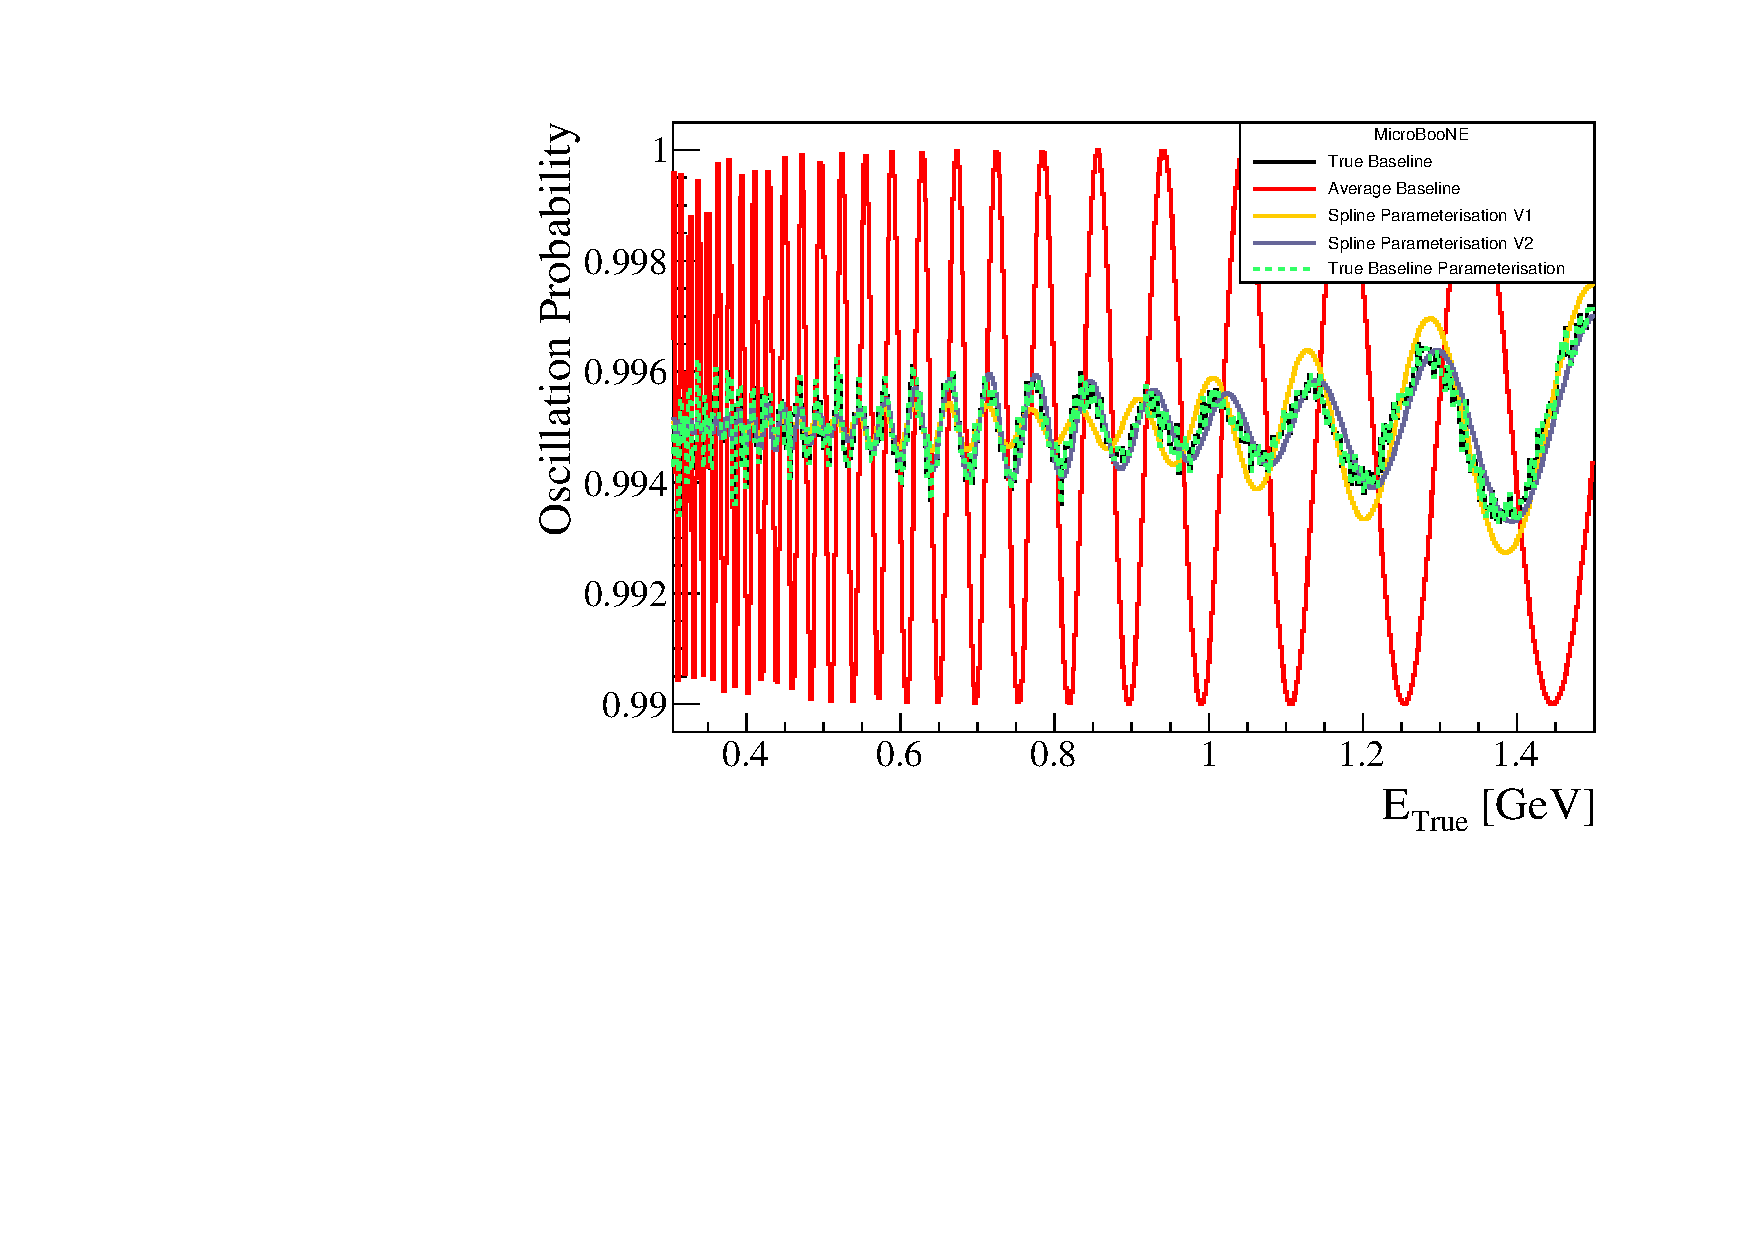
\includegraphics[width = 0.32\textwidth]{figures-chap5/osc_prob_uboone.pdf}
    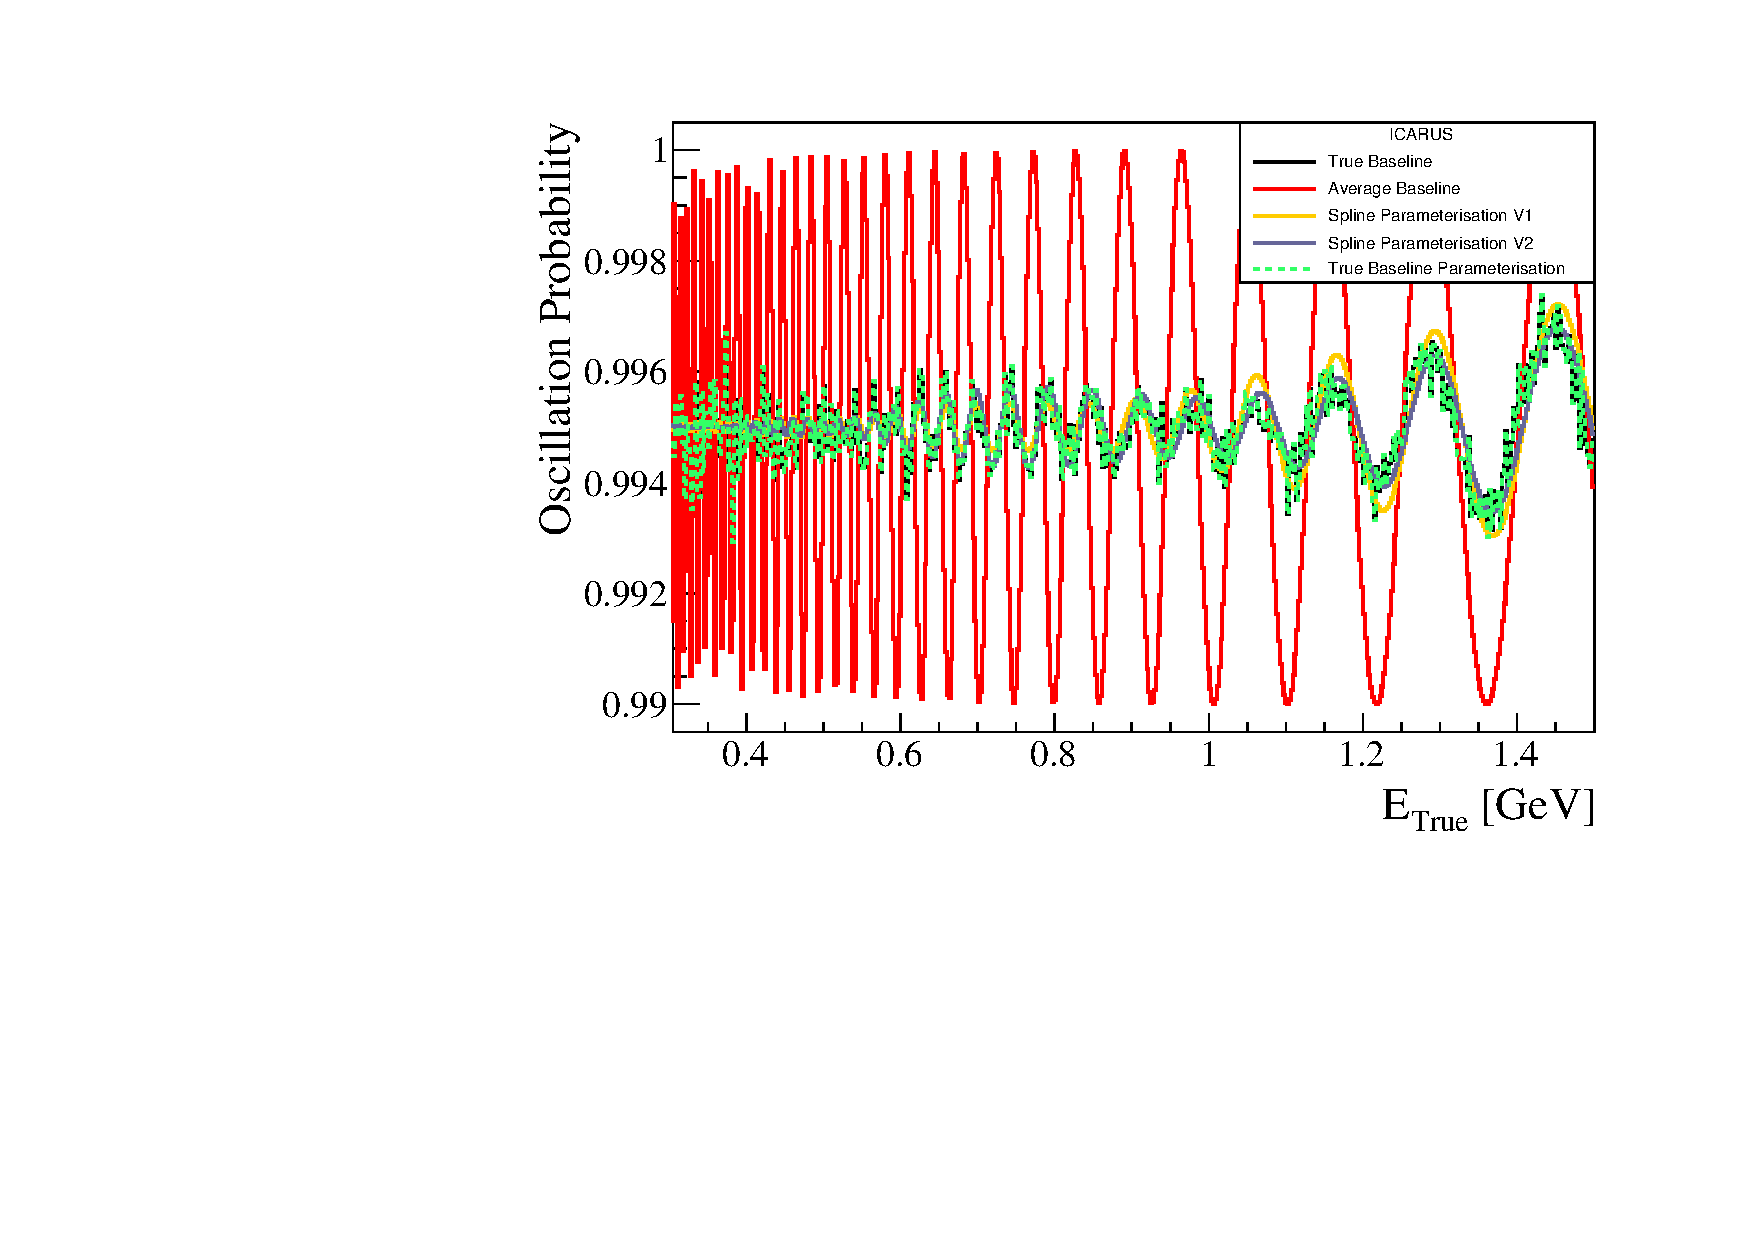
\includegraphics[width = 0.32\textwidth]{figures-chap5/osc_prob_icarus.pdf}
    \caption{The oscillation probability as a function of true neutrino energy for the \numu disappearance sample with oscillation parameters $sin^22\theta_{\mu\mu} = 0.01$ and $\Delta m^2_{41} = 50$ eV$^2$ in each \gls{sbn} detector. The results from using each baseline parametrisation are shown.}
    \label{fig:baseline_osc_probability}
\end{figure}

\subsection{Binning}\label{sec:binning}

The $\nu_\mu$ edge-to-edge binning has 21 bins in reconstructed neutrino energy which are bounded as follows:
\begin{itemize}
    \item 1 bin from 0.0-0.2 GeV,
    \item 2 0.1-GeV bins from 0.2-0.4 GeV,
    \item 12 0.05-GeV bins from 0.4-1.0 GeV,
    \item 2 0.25-GeV bins from 1.0-1.5 GeV,
    \item 3 0.5-GeV bins from 1.5-3.0 GeV and
    \item 1 bin from 3.0-10.0 GeV.
\end{itemize}

The $\nu_\mu$ edge-to-edge binning has 22 bins in true neutrino energy which are bounded as follows:
\begin{itemize}
    \item 1 bin from 0.00-0.30 GeV,
    \item 3 0.10-GeV bins from 0.30-0.60 GeV,
    \item 12 0.05-GeV bins from 0.60-1.20 GeV,
    \item 1 bin from 1.20-1.50 GeV,
    \item 3 0.50-GeV bins from 1.50-3.00 GeV,
    \item 1 bin from 3.00-5.00 GeV and
    \item 1 bin from 5.00-10.00 GeV.
\end{itemize}

The $\nu_e$ edge-to-edge binning has 12 bins in reconstructed neutrino energy which are bounded as follows:
\begin{itemize}
    \item 1 0.35-GeV bin from 0.00-0.35 GeV,
    \item 5 0.15-GeV bins from 0.35-1.10 GeV,
    \item 2 0.20-GeV bins from 1.10-1.50 GeV,
    \item 2 0.25-GeV bins from 1.50-2.00 GeV,
    \item 1 bin from 2.00-3.00 GeV and
    \item 1 bin from 3.00-10.00 GeV.
\end{itemize}

The $\nu_e$ edge-to-edge binning has 33 bins in true neutrino energy which are bounded as follows:
\begin{itemize}
    \item 2 0.25-GeV bin from 0.00-0.50 GeV,
    \item 15 0.05-GeV bins from 0.50-1.25 GeV,
    \item 15 0.25-GeV bins from 1.25-5.00 GeV and
    \item 1 bin from 5.00-10.00 GeV.
\end{itemize}

